\documentclass[12pt,a4paper]{jbook}
\usepackage{mm-thesis}
\usepackage[dvipdfmx]{graphicx}

\thesis{\master} 
%修士学位論文の場合は\master


\title{OS仮想化基盤を用いたSBCマルチディスプレイシステムのフレーム処理並列化}

\author{高畑 勇我}

\supervisor{下條 真司 教授}

\deadline{2022年2月9日}
%提出期限を書く. 

\abstract{
複数のディスプレイを1台の大型ディスプレイとして仮想化するマルチディスプレイシステム (MD) は,高解像な動画像を複数人で見る目的で利用される.
先行研究では,MD構築コストの低減を目的としてシングルボードコンピュータ (SBC) を用いたMDが提案された.
このMDはヘッドノードとディスプレイノードの2種類のノードから構成されており,SBCで実装したディスプレイノードの負荷を低減するためにヘッドノードで画像フレームの処理を行っている.
しかし,ヘッドノードで行われている処理がボトルネックとなり,高フレームレートまたは高解像度な動画を再生すると動画表示に遅延が発生する.
また,分割後のフレームごとに圧縮処理と送信処理を行うため,これらの処理を単一のプロセスで行う場合には処理の待ち時間が発生し,MDのパフォーマンスおよびスケーラビリティを低下させている.
本研究では,OS仮想化技術を利用し,ヘッドノードのフレーム圧縮部分を並列化し独立したプロセスとして実装することでフレームの処理時間を短縮し,MDのボトルネック解消を目指す.

提案手法におけるヘッドノードは,画像フレームの分割を行う分割コンテナ,画像フレームの圧縮と送信を行う圧縮コンテナ,ディスプレイノード群の同期制御を行う同期制御コンテナの3種類のコンテナで構成する.
分割コンテナおよび同期制御コンテナはそれぞれヘッドノード内に単一のプロセスとして動作する.
また,圧縮コンテナはMDを構成するディスプレイと同数が動作しており,対応するディスプレイノードと1対1で接続する.
分割コンテナと圧縮コンテナの間で必要となる画像フレームの受け渡し処理には,高速なプロセス間データ通信が可能な共有メモリ(SYSTEM V IPC)を使用し,
フレームデータ受け渡しにかかるオーバーヘッドを抑える.

評価では,提案手法によるヘッドノードでのフレーム処理時間の変化を確認するため,4K解像度の映像を用いてヘッドノードのフレーム処理に要する時間を計測,比較した.
ディスプレイ4面構成および9面構成のMDを動作させることを想定し,ヘッドノード内で1つの分割コンテナと,ディスプレイ数と同数の圧縮コンテナを動作させた.
評価結果より,4面構成時,9面構成時ともに提案手法ではフレーム処理に要する時間が短縮され,分散並列化によりシステムのボトルネックが解消されたことが確認できた.
また,ディスプレイ数を増加させても既存手法と比べて処理時間の増加は小さく,スケーラビリティも改善されていることが確認できた.


}

\keyword{マルチディスプレイ,小型低性能計算機,OS仮想化,コンテナ並列化,プロセス間通信}

\usepackage{float}
\usepackage{subfig}

\begin{document}

\coverpage

\tableofcontents

\body

\chapter{序論}

近年では,デジタル化の進展により大量のデータを取得できるようになり,それらのデータを活用して研究機関が行う学術研究が盛んになっている.
学術研究においては,個々の研究機関の枠組みを越えて研究設備や研究データを利活用することでより大きな成果が期待できる.
このような背景から,大学や研究機関の研究者たちによる共同研究のプロジェクト数が増加傾向にある~\cite{nisted,soumusyou}.

また,最近では新たなスーパーコンピュータの開発による計算能力の向上を背景に,シミュレーションベースで行われる研究・プロジェクトの数が増加している.KBDD (K supercomputer-Based Drug Discovery project by Biogrid pharma consortium) プロジェクト\cite{kbdd,kbddproject}は,新薬の開発を目指して立ち上げられた共同研究プロジェクトであり,タンパク質と化合物の結合可能性の予測に高性能計算機による大規模シミュレーションの結果が活用されている.国立研究開発法人海洋研究開発機構 (JAMSTEC) は,東京大学地震研究所と協力して「富岳」 \cite{fugaku}を用いた大規模数値シミュレーションによる地震・津波による複合災害の統合的予測システムを開発している \cite{jishin}.また,同様に「富岳」を用いて行われたCOVID-19の飛沫・エアロゾル拡散モデルシミュレーションに関する共同研究 \cite{covid-19}も記憶に新しい.

以上に挙げたような大規模シミュレーションを用いた共同研究では,行われたシミュレーションの結果を可視化し,複数人の研究者たちで議論を交わすことが必要となる.
そのため,複数人で同時に閲覧できるような大型の高解像ディスプレイが不可欠である.
高解像のディスプレイを構築する方法として,格子状に配置した複数のディスプレイを1台の仮想ディスプレイとして構成するマルチディスプレイシステム(MD)がある.
MDは4Kなどの高解像な動画や画像を大画面で表示することが可能であるため,多数の研究者らが議論する場などで利用される.
MDの導入事例を挙げると,大阪大学サイバーメディアセンターでは24面ディスプレイで構成されるMDを吹田本館に,15面のMDをうめきたVisLabに設置し運用しており,大規模シミュレーションやデータ同化シミュレーションの解析結果を可視化する高解像度ディスプレイとして活用している\cite{ciber_media}.
また名古屋大学情報基盤センターでは,16面MDを用いた可視化装置と連動する大規模情報システムを運用している\cite{nagoya}.

しかし,MDの構築および運用コストは高くなる傾向にある.
MDの構築方法には,主に2通りの手法が存在する.
まずマトリックススイッチャを用いたMD構築用ハードウェアを用いる方法であるが,可視化用途の専用機器は一般に高価であるため,MD構築にかかる費用が高くなる.
もう一方はSAGE2~\cite{sage2}などに代表されるMD構築用ミドルウェアを用いる方法である.
この手法では,ディスプレイに映像を出力するための計算機を複数台用意し,それらとは別の制御用の計算機を用意する構成となる.
ディスプレイを接続した計算機では,3Dレンダリングや描画を行うため,一般的に高価なグラフィックボードを用いる.
また,制御用計算機では画像もしくは可視化データの送受信が頻繁に発生するため,高性能なネットワーク機器が用いられる.
そのため,可視化用途の計算機の費用は高くなる.

こうしたMDの構築費用に関する問題に対して,先行研究でシングルボードコンピュータ(SBC)を用いて構築したMDが提案された.
先行研究で提案されたMDは,画像フレームの分割・圧縮・送信,通信の制御を行うヘッドノードと,分割された画像フレームを描画するディスプレイノードとで構成されている.
まず,ディスプレイノードにSBCを用いるため,ディスプレイノードに高負荷な処理が要求されないようフレーム転送方式による連携表示処理を行っている.
ヘッドノードはフレームの分割および圧縮を行ってからフレームを送信し,ディスプレイノードが圧縮済フレームを受信し展開することで動画をディスプレイ上に表示する.

しかし,このMDではヘッドノード内でのフレーム処理を単一のプロセスで行っているため,高解像度な動画や高フレームレートな動画を表示する場合には動作に遅延が生じる.
また,MDの構成ディスプレイ数を増加させた場合にも動作遅延が生じるため,スケーラビリティにも問題を抱えている.
そこで本研究では画像フレームの圧縮を行うプロセスを構成ディスプレイと同じ数だけ用意し,ヘッドノード内で並列化してフレーム圧縮処理を行う手法を提案する.
フレーム処理の並列化はOS仮想化基盤を利用し,プロセスをコンテナとして動作させることで実現する.
フレーム処理の並列化を行うことで,ヘッドノード内でのフレーム処理時間を短縮とMDのスケーラビリティ向上を目指す.

以下,本論文の構成について述べる.
2章では,主なマルチディスプレイシステムの構築方法について説明し,低価格なマルチディスプレイ構築方法の重要性について述べる.また,ディスプレイノードにSBCを用いて構築された先行研究を紹介し,その関連研究として自身の卒業研究にも触れる.
3章では,本研究の目的を実現するための提案手法である,OS仮想化技術を用いたヘッドノードのフレーム処理並列化について説明し,その設計と実装,関連技術について詳細に説明する.
4章では,提案手法の効果を確認するための評価実験について述べる.
5章では,仮想化技術を用いてマルチディスプレイシステムを構築した関連研究について述べる.
最後に6章で本研究を総括し,今後の課題点について述べる.

\chapter{小型低性能計算機を用いたマルチディスプレイシステムの構築}

本章では,小型低性能計算機,特にSBCを利用した低コストなマルチディスプレイシステム構築手法の必要性と,その実現に向けて行われた先行研究について説明する.
まず2.1節では,従来利用されてきたマルチディスプレイシステムの構築手法とそのコストについて述べる.
続く2.2節では,先行研究でも使用されており,本研究でも取り扱うシングルボードコンピュータ (SBC) について説明し,2.3節では先行研究である,SBCを用いて構築されたマルチディスプレイシステムについて説明する.
さらに2.4節で,先行研究で提案されたSBCを用いたマルチディスプレイシステムについての問題点と,その問題点を解決することを目的として行われた関連研究を紹介する.
最後に2.5節では関連研究において将来的な課題とされていた部分の改善策と,それを実現するための技術的な課題点について述べる.

\section{従来のマルチディスプレイ構築手法}
これまでMDの構築には数多くの手法が提案されており,それらは大きく分けると2種類の手法に分類することができる\cite{pccluster,6693038}.
1つはマルチディスプレイを構築可能にする専用のハードウェアを用いて構築する手法であり,もう1つはマルチディスプレイを構築可能にする専用のミドルウェアを用いて構築する手法である.
本節では,この2種類の構築手法を簡単に解説してそれぞれの構成例を示し,構築に要する金銭的コストについて説明する.

\subsection*{専用ハードウェアを用いたマルチディスプレイの構築}

マルチディスプレイ構築用のハードウェアは接続した複数台のディスプレイに対して映像出力用の信号を送信する機能を持った機器であり,主にデジタルサイネージ\cite{signage}や会議用のディスプレイを構築する際に利用される.
マルチディスプレイ構築用ハードウェアの多くは,HDMI (High-Definition Multimedia Interface), DisplayPort \cite{displayport}等の規格に対応した映像出力ポートを複数搭載しており,各ポートに映像信号を分配することによって,接続したディスプレイを連動させて制御する.
マルチディスプレイ構築用ハードウェアは,表示映像フレームの分割,接続ディスプレイ間の同期処理などをハードウェアレベルで行う.
ハードウェアベースで処理を行うことにより高速なフレーム処理が可能となり,ディスプレイ上に高フレームレートで映像を出力することができる.
一方で,マルチディスプレイ構築用ハードウェアは入力ポート,出力ポートそれぞれの設置数が固定であるため,入出力に使用できるポート数には上限が存在することになる.
そのため,マルチディスプレイを構築するディスプレイ数にも上限が存在することになり,より大規模なディスプレイや高解像なディスプレイを構築する事が難しい.これがマルチディスプレイシステムのスケーラビリティという観点からすると欠点となっている.
マルチディスプレイシステム構築用ハードウェアの具体例としては,グラフィックボードやマトリックススイッチャが存在する.
図\ref{fig_2.1}に,マトリックススイッチャを用いて構築したマルチディスプレイの概要図を示す.

\begin{figure}[htbp]
 \includegraphics[width=1.02\linewidth]{./fig/chap2/matrixswitcher.eps}
 \caption{専用ハードウェアを用いたマルチディスプレイシステム}
 \label{fig_2.1}
\end{figure}

グラフィックボードは,PCなどのコンピュータにおいて,映像を信号として入出力するための機能を拡張ボードとして独立させたものである.
また,一般的には内部にGPU (Graphics Processing Unit) と呼ばれるグラフィックスを描画する際の計算処理を行う半導体チップが組み込まれており,高速な画像処理が可能である.
各グラフィックボードに搭載されているチップやメモリによって,描画可能な解像度や表現色数,2D/3D描画性能などが異なる.
マルチディスプレイを構築する目的でグラフィックボードを使用すると,ある程度の高解像な画像を描画可能であり,信号の入出力可能ポート数が多層備え付けられているものが必要となる.
マルチディスプレイ対応型のグラフィックボードは,NVIDIA社やAMD社から発売されている.
マルチディスプレイ対応型のグラフィックボードは,一般的に利用可能な映像出力ポート数が多く,表示解像度が優れているものほど価格が高くなる.

\subsection*{専用ミドルウェアを用いたマルチディスプレイシステム}

マルチディスプレイ構築用ミドルウェアは,ディスプレイに接続した汎用PCに画像フレームまたは描画命令を送信することによって動画や画像を表示する.
マルチディスプレイ構築用ミドルウェアは主に科学的可視化の分野で広く利用されており,高性能なコンピュータで行われたシミュレーションの結果を表示する大規模可視化装置の構築などに使用される.
接続可能なディスプレイ数に上限は設けられておらず,多数の汎用PCを連携して動作させることでスケーラブルなマルチディスプレイの構築が可能である.
しかし,マルチディスプレイ構築用ミドルウェアは大規模な科学的可視化の用途を想定して設計されたものが多く,ディスプレイと接続された汎用PC群に対して高負荷な描画処理を要求するものが多い.
そのため,マルチディスプレイを構築するために使用される汎用PCには一定の処理性能を満たすものが必要となり,マルチディスプレイを構成するディスプレイ数が増加するごとに構築費用が高騰するという問題点がある.
図\ref{fig_2.2}に,マルチディスプレイ構築用ミドルウェアを用いて汎用PC群を連携させることで構築したマルチディスプレイの構成例を示す.

\begin{figure}[htbp]
 \includegraphics[width=1.02\linewidth]{./fig/chap2/middleware.eps}
 \caption{マルチディスプレイ構築用ミドルウェア}
 \label{fig_2.2}
\end{figure}

それぞれのPCはマルチディスプレイ構築用ミドルウェアによってヘッドノードまたはディスプレイノードとして動作することが可能になる.
ヘッドノードは各ディスプレイに画像を表示するための信号の送信やヘッドノード-ディスプレイノード間の同期処理などの役割を担う.
ディスプレイノードはマルチディスプレイを構築するディスプレイに接続され画像の描画や表示に関する計算や処理を行う.
ディスプレイノードとディスプレイは1対1で接続されるため,ディスプレイノードはマルチディスプレイを構築するディスプレイの数と同数用意する必要がある.

以下,専用ミドルウェアを用いたマルチディスプレイシステムの詳細な動作について説明する.
各ミドルウェアによって行われる連携表示処理には,大きく分けて2通りの手法がある.
1つはフレーム転送方式と呼ばれる手法である.
フレーム転送方式はヘッドノードがディスプレイノードに対して表示映像のフレームを送信し,ヘッドノードとディスプレイノードの同期処理によってフレームをディスプレイ上に連携表示させる方式である.
フレーム転送方式を採用するマルチディスプレイの例として,SAGE \cite{sage}やSAGE2 \cite{sage2}などがあげられる.

フレーム転送方式は,以下の5種類の動作から成り立つ.

\begin{itemize}
    \item フレーム圧縮
    \item フレーム送信
    \item フレーム展開
    \item 同期制御
    \item フレーム表示
  \end{itemize}

まずヘッドノード上で表示映像からフレームが切り出され,フレームの圧縮処理が行われる.
このとき,フレームを各ディスプレイノードの表示領域に合わせて分割する手法と,フレーム全体をそのまま圧縮する手法の2通りが存在する.
前者はSAGE \cite{sage},後者はDisplayCluster \cite{displaycluster}といったミドルウェアでそれぞれ採用されている.
フレームの圧縮にはDXT (DirectX Texture Compression) \cite{dxt}やJPEG (Joint Photographic Experts Group) \cite{jpeg}などが利用される.

続いて,ヘッドノードで圧縮されたフレームを各ディスプレイノードへ送信する.
ディスプレイノードは,ヘッドノードから圧縮フレームを受信したあと展開処理を行い,続いて同期処理を開始する.
同期処理では,まずフレームの展開を終え表示待機状態になったディスプレイノードからヘッドノードへ表示準備完了通知が送信される.
ヘッドノードは,接続された全てのディスプレイノードから表示準備完了通知を受け取った後,各ディスプレイノード宛に表示命令を送信する.
表示命令を受け取ったディスプレイノードは,該当フレームをディスプレイ上に表示する.
この一連の動作を繰り返し行うことで,ディスプレイ上に連携して動画を表示することが可能になる.

もう1つは,描画命令転送方式と呼ばれる方式である.この方式では,ヘッドノードはディスプレイノードに対して画像フレームの送信を行わず,アプリケーションの出力する描画命令を同期処理を行いつつ送信することで動画の連携表示を行う.この方式を採用しているミドルウェアとしては,DMX (Distributed Multihead X) やChromium \cite{chromium}などがあげられる.

描画命令転送方式は,主に以下の4種類の動作から成り立つ.

\begin{itemize}
    \item 描画命令のキャプチャリング
    \item 描画命令転送
    \item 同期制御
    \item フレーム描画
\end{itemize}

  まず,ヘッドノードはアプリケーションから出力された描画命令のキャプチャリングを行う.
  続いて,ヘッドノードがキャプチャリングした描画命令をディスプレイノードへ送信する.
  描画命令を受信したディスプレイノードは,命令を受け取ったことを通知するメッセージをヘッドノードへ送信する.
  ヘッドノードは全てのディスプレイノードから描画命令受信通知を受信し次第,フレーム描画命令を送信し,ディスプレイノードがこの描画命令を受信しディスプレイ上にフレームを描画する.
  この一連の動作を繰り返し行うことで,ディスプレイ上に連携して動画を表示する.

\section*{シングルボードコンピュータ(SBC)}

シングルボードコンピュータ(SBC)は,1枚の基板上に必要最低限の部品を取り付けることで構築された小型計算機である.
SBCは他の汎用PCと比較しても非常に低価格で手に入れることができ,消費電力も少ないため,IoT (Internet of Things) 向けの機器として一般に利用される\cite{130007722836,7380571}.
また,軽量プログラミング言語が利用できることから,教育用やプログラミング学習用としても使用されている.
SBCにはRaspberry Piシリーズを代表として,様々な種類のものが存在する.
表\ref{table_2.1}に主なSBCの機種とその仕様を示す.
また,図\ref{fig_2.3}に主なSBCの画像を示す.

\begin{table}[H]
  \caption{SBC機種の仕様および価格}
  \begin{center}
  \begin{tabular}{cccc}
  \hline
  機種 & \begin{tabular}{c}Raspberry Pi 4 \\ Model B \cite{model4B} \end{tabular} & \begin{tabular}{c}Orange Pi \\ Zero Plus2 \cite{orengepi} \end{tabular} & \begin{tabular}{c} Banana Pi \\ BPI-M64 \cite{bananapi} \end{tabular}\\ \hline\hline
  CPU & \begin{tabular}{c}ARM Cortex-72 \\ (1.5 GHz×4)\end{tabular} &  \begin{tabular}{c}ARM Cortex-A53 \\ (1.8 GHz×4) \end{tabular} & \begin{tabular}{c} ARM Cortex-A53 \\ (1.2 GHz × 4) \end{tabular} \\ \hline
  GPU & \begin{tabular}{c}Broadcom VideoCore \\ IV (500 MHz) \end{tabular} & \begin{tabular}{c} Mali T720MP2 \\ (650 MHz) \end{tabular} & \begin{tabular}{c} Mali-400 MP2 \\ (500 MHz) \end{tabular} \\ \hline
  メモリ & 4.0 GB & 4.0 GB & 8.0 GB \\ \hline
  通信帯域 & 1 Gbps & 100 Mbps & 1 Gbps \\  \hline
  映像出力端子 & HDMI × 2 & HDMI × 1 & HDMI × 1 \\ \hline
  OS & Linux & Linux & Linux \\  \hline
  価格 & 約8,000円 & 約14,000円 & 約9,000円 \\ \hline

  \end{tabular}
  \label{table_2.1}
  \end{center}
\end{table}


\begin{figure}[htbp]
  \begin{center}
    \begin{tabular}{c}

      % 1
      \begin{minipage}{0.33\hsize}
        \begin{center}
          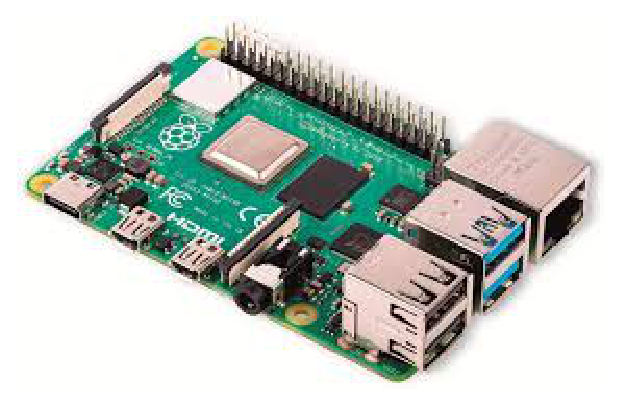
\includegraphics[clip, width=4.5cm]{./fig/chap2/raspi4b.eps}
          \hspace{1.6cm} Raspberry Pi Model 4 B \cite{model4B}
        \end{center}
      \end{minipage}

      % 2
      \begin{minipage}{0.33\hsize}
        \begin{center}
          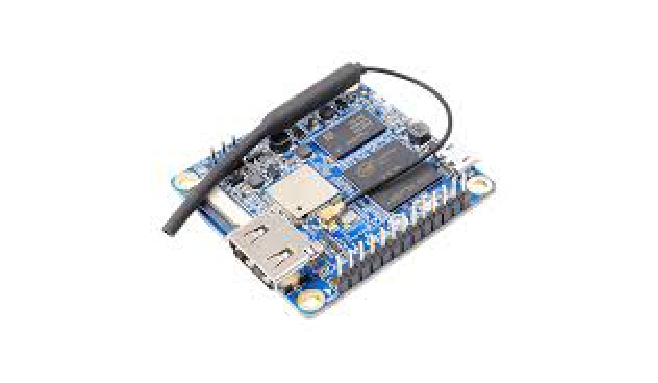
\includegraphics[clip, width=6.0cm]{./fig/chap2/orenge_pi.eps}
          \hspace{1.6cm} Orange Pi Zero Plus2 \cite{orengepi}
        \end{center}
      \end{minipage}

      % 3
      \begin{minipage}{0.33\hsize}
        \begin{center}
          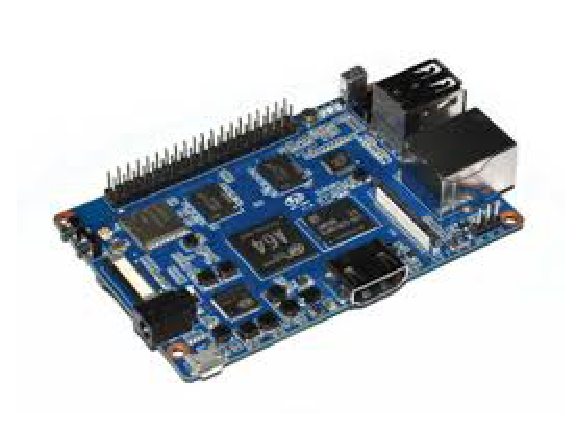
\includegraphics[clip, width=4.5cm]{./fig/chap2/banana_pi.eps}
          \hspace{1.6cm} Banana Pi BPI-M64 \cite{bananapi}
        \end{center}
      \end{minipage}

    \end{tabular}
    \caption{主なSBCの画像}
    \label{fig_2.3}
  \end{center}
\end{figure}



SBCが持つCPUの特徴は,主に低周波数のコアがデュアルコア,クアッドコアなどの形式で複数搭載されているものが多いことである.
低周波数コアの複数搭載は消費電力を抑えるため,また価格を低く抑えるためであり,こうした省電力や低価格という特徴を維持しつつCPU自体の処理能力を向上させる目的で,近年ではコア数の増加が進んでおり,マルチコア方式を採用した機種が多く販売されるようになってきている.
搭載メモリや通信帯域に関しては,近年のSBCの性能向上により4.0 GB以上の比較的大きなメモリ容量を持つものも増えており,ギガビットイーサネットに対応したNIC (Network Interface Card) を有するものも多く発売されるようになってきている.
映像出力の機能としては,ほとんどの機種でHDMI端子による出力が可能であり,Full HD 解像度での出力が標準的である.
また,各機種のOSには軽量なLinuxベースのOSが広く採用されている.
例えばRaspberry Piに対応したOSであるRaspbian \cite{raspbian}もLinuxをベースとするOSの一種である.



\section{先行研究で提案されたマルチディスプレイシステム}

2.1節で述べたように,ハードウェアを用いたマルチディスプレイの構築ではハードウェア自体の価格によりマルチディスプレイシステムの構築コストが増大する.
また,ミドルウェアを用いてマルチディスプレイシステムを構築する場合でも,ディスプレイと1対1で接続して映像の表示を制御する役割を持った
ディスプレイノードとして動作する汎用PCが複数台必要になるため同様に構築コストが増大する.
このようなマルチディスプレイシステム構築におけるコスト面の問題に対して,マルチディスプレイシステムの構築費用を低減する目的でディスプレイノードとしてSBCを活用するミドルウェアの開発が行われた.

本節では,先行研究 \cite{Ishida}で提案された,SBCを用いて構築されたマルチディスプレイの特徴について述べる.
まず,マルチディスプレイを構築する各ノードの動作について説明する.
その後フレームの連携表示処理を可能にする仕組みについて概説する.

\subsection*{連携表示処理}

先行研究で構築されたマルチディスプレイシステムは,1台のヘッドノードと,SBCを用いて実装された複数台のディスプレイノードで構成されている.

システムの概要を図2.4に示す.

\begin{figure}[H]
  \hspace*{\fill}
  \includegraphics[width=\linewidth]{./fig/chap2/system_4.eps}
  \hspace*{\fill}
  \label{fig_2.4}
  \caption{SBCを用いて構築したシステムの概要図}
 \end{figure}

このマルチディスプレイシステムは,2.1節で述べた2種類の方式のうち,フレーム転送方式を採用している.
そのため,SBCをディスプレイノードとして用いることとなり,従来のフレーム転送方式をそのまま適用するとSBC上で負荷の高い処理を行う必要がある.
しかし,SBCは市販の汎用PCなどと比べると処理速度,描画性能などの面で劣っているため,可能な限りディスプレイノード上での処理負荷を小さく抑えなければならないという制約が存在する.
そのため,SBCがディスプレイノードとして十分高速に動作するような設計を目的として,JPEG圧縮や連携表示処理のパイプライン化などが実装されている.

以下では,先行研究において提案されたマルチディスプレイシステムの詳細な動作について述べる.
ヘッドノードでは,動画ファイルからフレームを切り出した後,接続ディスプレイノード数に応じてフレームの分割を行う.
分割したフレームはそれぞれJPEG方式で圧縮され,各ディスプレイノードへと送信される.
ヘッドノードから送信された圧縮フレームを受信したディスプレイノードでは,フレームを展開し,その展開が終了した後表示バッファに格納してヘッドノードに表示準備完了メッセージを送信する.ヘッドノードは全てのディスプレイノードからの表示準備完了メッセージを受け取り次第表示命令を送信し,命令を受け取ったディスプレイノードはディスプレイ上にフレームを表示する.

また,ノード上の各処理はスレッド処理によって行われており,ヘッドノード上では圧縮スレッド,送信スレッド,同期制御スレッドの3種類,ディスプレイノード上では受信スレッド,展開スレッド,表示制御スレッドの3種類のスレッドが動作している.

各スレッドの操作を図2.5に示す.

圧縮スレッドは,表示映像の切り出しと分割,圧縮までを行う.
送信スレッドは,圧縮されたフレームを各ディスプレイノードに送信する.
同期制御スレッドは,表示準備完了メッセージの受信と表示命令の送信を行う.
受信スレッドは,ヘッドノードから圧縮フレームを受信する.
展開スレッドは,圧縮フレームの展開を行う.
表示スレッドは,ヘッドノードからの表示命令を受け取りフレームをディスプレイ上に表示する.

\begin{center}
  \begin{figure}[H]
      \hspace*{\fill}
      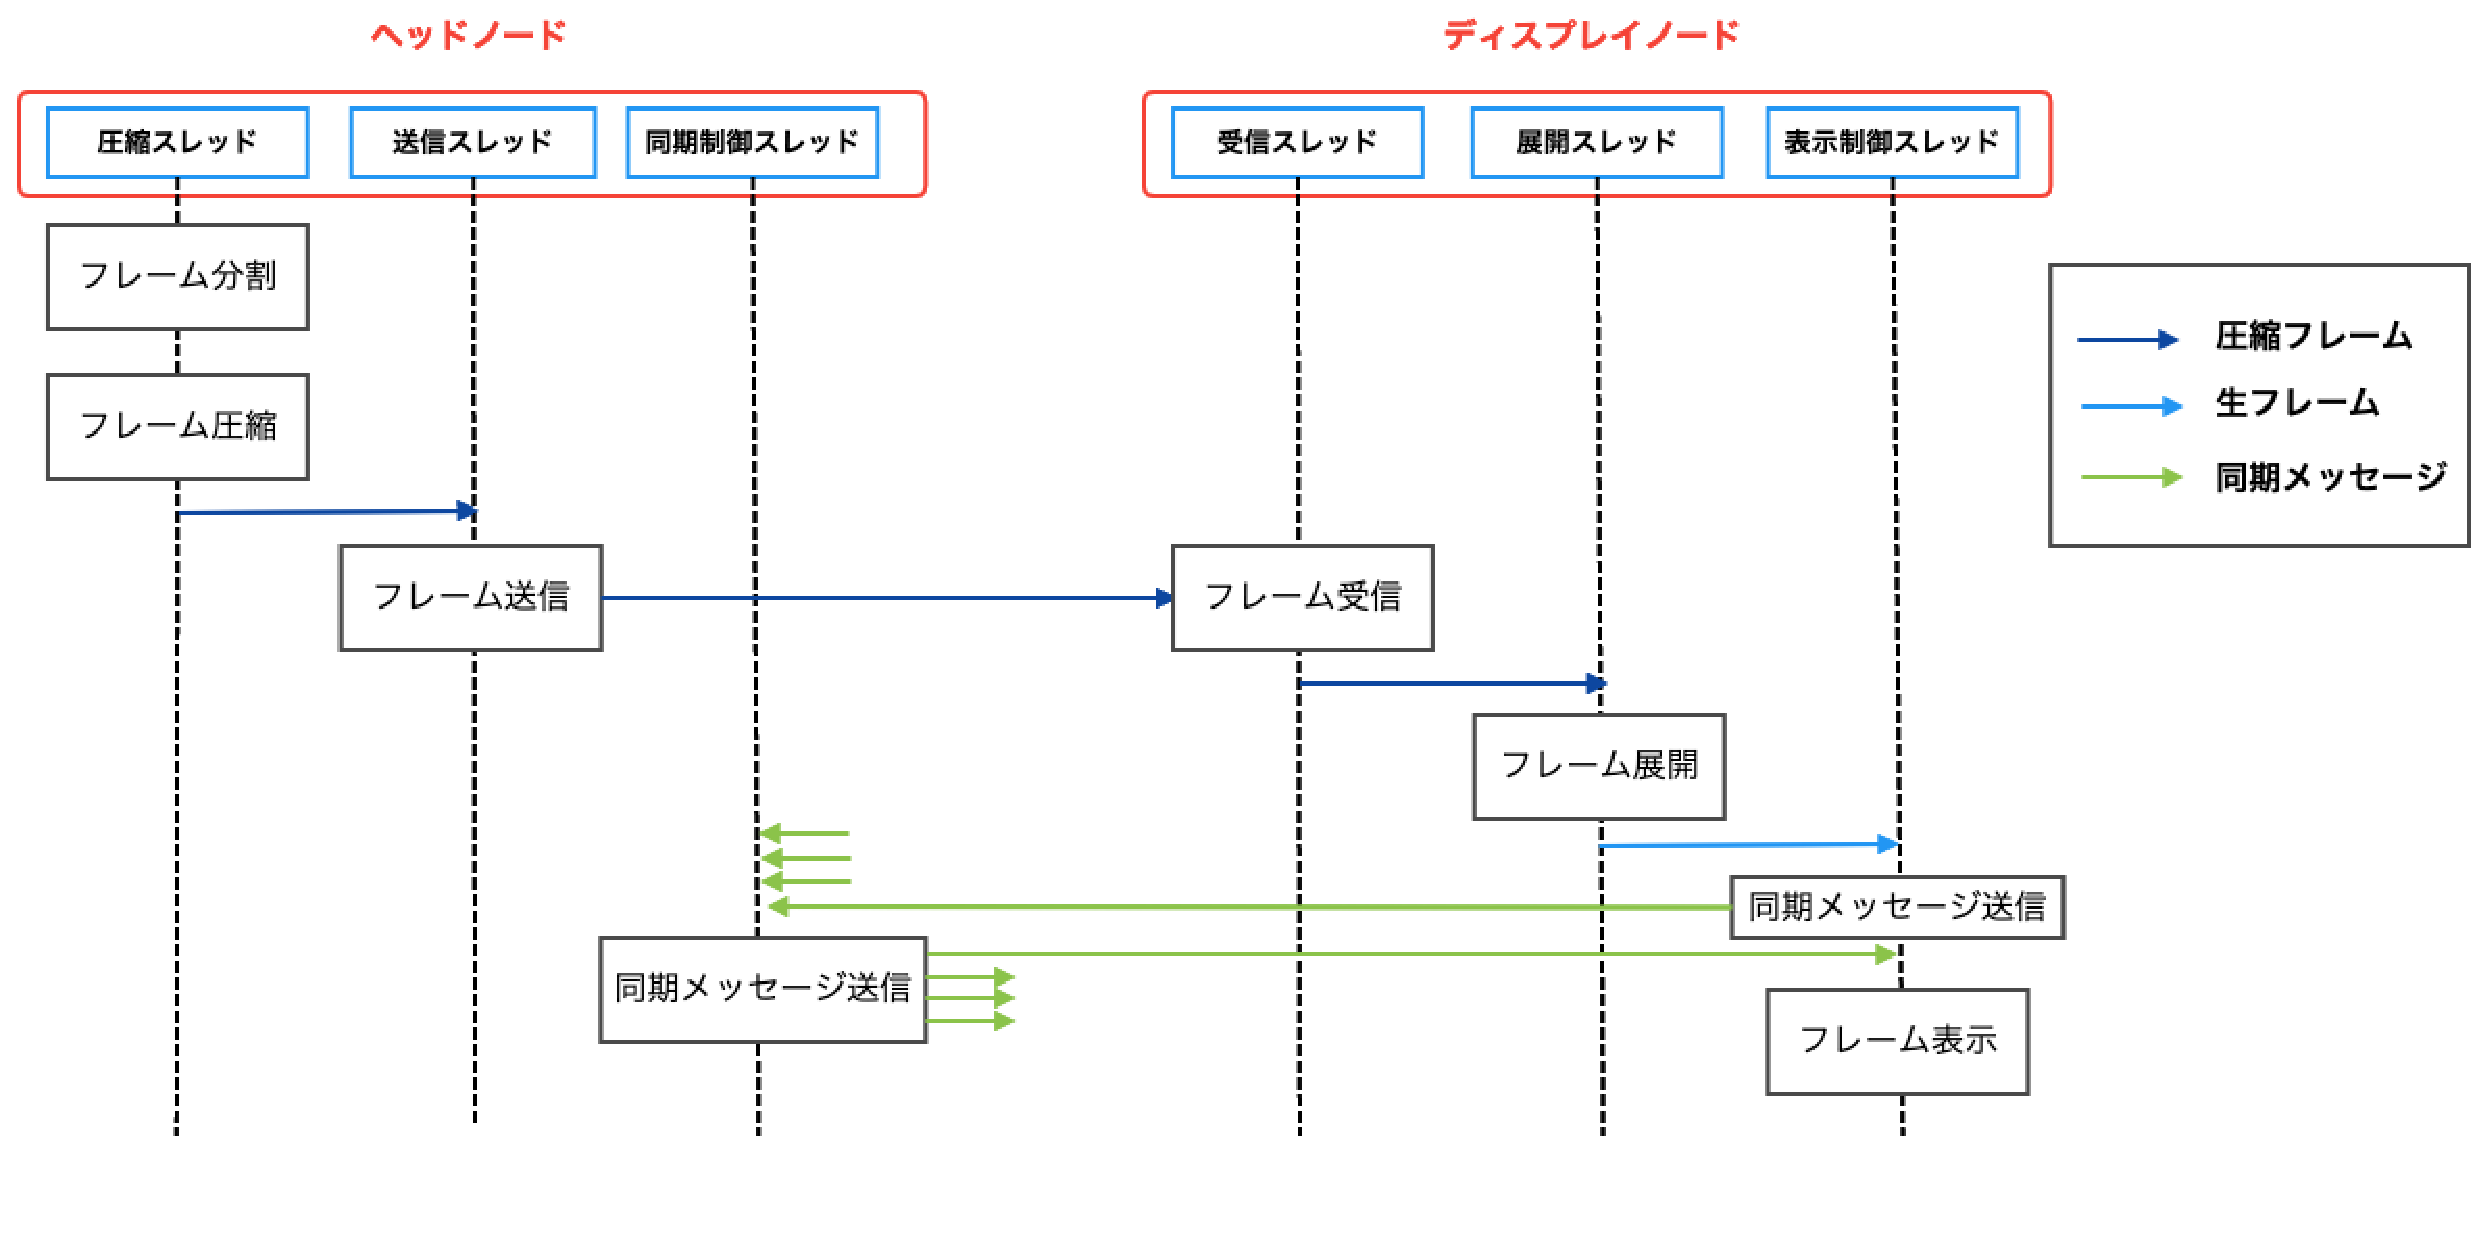
\includegraphics[width=1.1\linewidth]{./fig/chap2/frow_system.eps}
      \hspace*{\fill}
      \caption{各スレッドの動作}
  \end{figure}
  \end{center}

  \begin{center}
    \begin{figure}[H]
        \hspace*{\fill}
        \includegraphics[width=1.1\linewidth]{./fig/chap2/previous_thread.eps}
        \hspace*{\fill}
        \caption{各スレッドの動作}
    \end{figure}
    \end{center}
   

\subsection*{フィードバック処理}

JPEG圧縮処理では,まず入力画像のピクセルごとの画素値をRGB形式からYCbCr形式に変換する.
YCbCrは色彩表現法の一種であり,色を人間の目が認識しやすい輝度成分と認識しづらい色差成分とに分けて表現する\cite{YCbCr}.
YCbCr形式に変換された色成分はデータ量を削減するために間引かれることになるが,この時YCbCrサンプル比という間引き方を決定するパラメータを変更することで,
JPEG圧縮に要する時間を変更することができる~\cite{jpeg2}.
また,量子化を行う際の品質係数と呼ばれるパラメータを変更することによっても,JPEG圧縮に要する時間を短縮することができる.
先行研究のマルチディスプレイシステムでは,ディスプレイノードで動画再生時のフレームレートを計算し,目標フレームレートとの差に応じてこれらのパラメータを変更することで,フレームレートを目標値に近づけるフィードバック処理を実装している.





\section*{問題点と技術的課題}

本節では,前節で述べた先行研究におけるマルチディスプレイシステムの問題点と,それを解決するための技術的課題について述べる.
まず,先行研究のマルチディスプレイシステムにおける具体的な問題について説明する.その後,問題点解決に向けた手法の考察と利点,欠点について述べ,比較を行う.

\section*{先行研究で提案されたマルチディスプレイシステムの問題点}
先行研究で構築されたマルチディスプレイには,高解像度な動画や高フレームレートな動画を表示しようとするとパフォーマンスが低下するという問題点がある.
この問題の原因となっているのが,ヘッドノードでのフレーム処理である.
前述したように,ヘッドノード内では動画フレームに対して分割,圧縮,送信の3つの処理が行われている.
高解像度な動画では1フレームあたりのデータ量が大きくなるためフレームの圧縮に時間がかかり,パフォーマンスが低下する.
また,高フレームレートな動画ではフレーム圧縮に要する時間が動画における1フレームの表示時間を上回り,動画本来のフレームレートを維持したまま動画を再生することが困難になる.

また,大規模なマルチディスプレイを構築した際のパフォーマンス低下も問題点として挙げられる.
先行研究で構築されたMDの中では圧縮スレッド,送信スレッド,同期制御スレッドがそれぞれ1つのスレッドとして動作している.
マルチディスプレイを構成するディスプレイの数が増加した場合にはそれに伴ってフレーム圧縮処理の回数も増加し,圧縮スレッドでのフレーム処理負荷も同様に増加することとなる.
しかし,ヘッドノード内で動作する圧縮スレッドは1つであるため,処理負荷の増加に伴って処理に要する時間も増加することとなり,動画再生時のフレームレート低下につながる.
実際,4面構成の場合では30fpsの動画をMD上に20〜22fpsで再生することが可能だが,ディスプレイを9面構成にしたMDでは8〜10fpsに低下することが確認できる(図2.6).

\begin{figure}[H]
  \hspace*{\fill}
  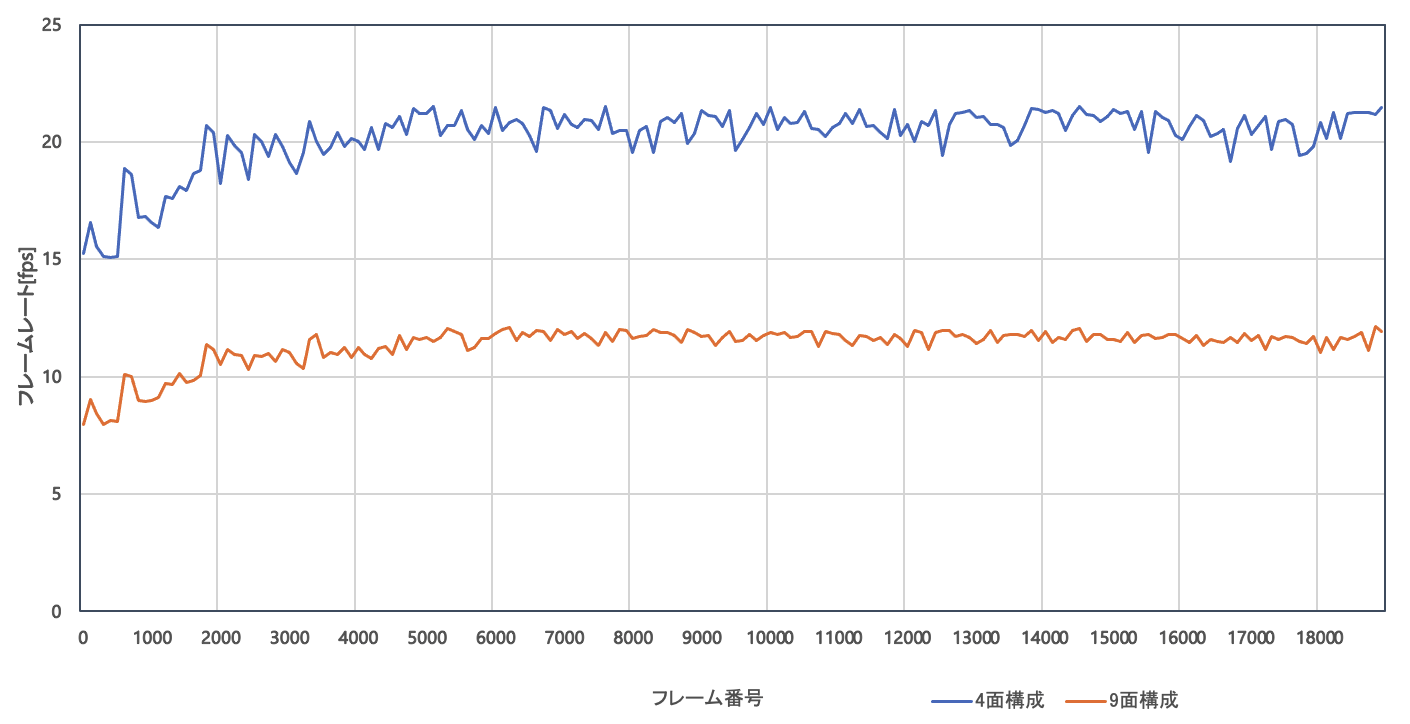
\includegraphics[width=\linewidth]{./fig/chap2/49.eps}
  \hspace*{\fill}
  \label{fig_2.6}
  \caption{画面構成変更時のフレームレート比較}
 \end{figure}


 \section{ヘッドノードの処理負荷軽減を行った関連研究}
 
ヘッドノード上でのフレーム処理負荷が増加しフレームレートが低下するという問題に対して有効な対策として,ヘッドノード上でのフレーム処理を並列化することにより処理負荷を軽減し,フレーム処理に要する時間の短縮を試みる手法が考えられる.
この手法を用いた関連研究として,自身の卒業研究がある.

\subsection*{実装の概要}

関連研究では,ヘッドノード上での処理を分散並列化する目的で,処理のノード分散を行っている.
ノード分散では,新たにノードとしてCPUを追加実装することによって物理的にCPUを増加させ,高負荷なフレーム処理を複数のCPUで分担して実行する.
また,ヘッドノードの性能に依存することが少なくなるため,ヘッドノードとしてCPUコア数が少ないような比較的低価格なPCを用いた場合にも大きく性能を落とさずに動作することが期待できる.

関連研究では,ヘッドノードの処理を複数のノードに分散するために,ヘッドノードとディスプレイノードとの間に新たにSBCを用いて中継ノードを実装した.
また,連携表示処理の並列化を行うため,中継ノード上での処理を受信スレッド,画像処理スレッド,送信スレッドという3種類のスレッドで分担して行うようマルチスレッド化している.

各スレッドの動作を図2.7に示す.

\subsection*{中継ノードの動作}
受信スレッドはヘッドノードから送信される一次分割済み非圧縮画像フレームを受信し,受信バッファへの格納を行う.
分割・圧縮スレッドは受信バッファに格納された非圧縮フレームを取り出し,接続されているディスプレイノードの数に応じてフレームの二次分割処理を行う.
その後,それぞれの分割済フレームに対してJPEG圧縮処理を行い,送信バッファへと格納する.
送信スレッドは,送信バッファに格納されたJPEG圧縮済フレームを,各接続ディスプレイノードへと送信する処理を行う.
以上の3種類のスレッドによって,中継ノードはヘッドノードとディスプレイノードとの間で連携表示処理を実現する.

\begin{figure}[H]
  \hspace*{\fill}
  \includegraphics[width=\linewidth]{./fig/chap2/frow_middle.eps}
  \hspace*{\fill}
  \caption{各スレッドの動作}
\end{figure}

\subsection*{ヘッドノードの動作}
中継ノードを実装したマルチディスプレイシステムでは,ヘッドノードは接続中継ノード数に応じて画像フレームの分割を行う.
分割された画像フレームは,送信スレッドへ渡され,各フレームに対してフレーム番号が付与される.
そして,フレーム番号の付与が終了したフレームは圧縮処理を行わずに中継ノードへと送信され,中継ノードは非圧縮フレームを受信して受信バッファに格納する.
その後,画像処理スレッドが非圧縮フレームを受信バッファから取り出し,接続ディスプレイノード数に応じて分割し,パラメータに従いJPEG形式に圧縮してディスプレイノードへ送信する.

\subsection*{ディスプレイノードの動作}
ディスプレイノードは中継ノードから送信された圧縮フレームを受信し,受信バッファに格納する.
その後,展開スレッドが圧縮フレームを展開する.
展開処理が終了したフレームは表示バッファに格納され,表示制御スレッドがこれを認識してヘッドノードへ表示準備が完了した旨の同期メッセージを送信する.
そして,ヘッドノードからの表示命令を受信し,表示制御スレッドが表示フレームの切り替えを行うことにより順次フレームがディスプレイ上に表示される.
この一連の動作を繰り返すことにより,マルチディスプレイシステムとしての連携表示処理が可能となる.

図3.2に提案手法を用いて構成した4面構成のマルチディスプレイシステム全体の論理構成図と動作フロー図を示す.


\begin{figure}[H]
  \hspace*{\fill}
  \includegraphics[width=\linewidth]{./fig/chap2/system_figure.eps}
  \hspace*{\fill}
  \caption{関連研究で提案された手法を用いたMDの動作フロー}
 \end{figure}

 \subsection*{関連研究の問題点と将来課題}
 ヘッドノードとディスプレイノードの間に中継ノードを実装してフレーム処理の分散並列化を図った関連研究では,ヘッドノードの高負荷状態を解消する事ができた.
 しかし,フレームレートなどシステムのパフォーマンスの面では,元々のマルチディスプレイシステムと比較して性能が低下した (表2.2).

 \begin{table}
  \centering
  \caption{中継ノード実装によるフレームレートの比較}\label{tab1}
  \scalebox{1.2}{
  \begin{tabular}{cccc}
  \hline
  手法 & 平均 & 最大 & 最小\\
  \hline
  中継ノード実装システム & 1.95 & 2.25 & 1.85\\
  中継ノード非実装システム & 9.44 & 10.42 & 7.35\\
  \hline
  \end{tabular}
  }
  \end{table}

 原因として考えられるのは,中継ノードを新たに実装したことで生じたフレームの送受信処理である.
 関連研究で提案されたマルチディスプレイシステムでは中継ノード内で画像フレームの圧縮処理を行うため,画像フレームはまずヘッドノードから中継ノードへと送信され,中継ノードで圧縮処理がなされた後ディスプレイノードへと送信される.
 この2度のフレーム送受信処理によって生じるオーバーヘッドが影響し,システムのパフォーマンスが低下したと考えられる.

 \section{関連研究での技術的課題}
関連研究の結果から,ヘッドノードの処理を外部のノードへ分散させる手法は画像フレームデータの送受信のオーバーヘッドが生じるためパフォーマンスの向上への貢献度が低い事がわかった.
フレームデータ送受信のオーバーヘッドを生じさせずにフレーム処理の並列化を行うためには,ヘッドノード内のCPUリソースを活用する事が必要である.

図2.9に,関連研究のヘッドノードにおけるCPU使用率の推移を示す.

\begin{figure}[H]
  \hspace*{\fill}
  \includegraphics[width=\linewidth]{./fig/chap2/cpurate_head_proposed.eps}
  \hspace*{\fill}
  \caption{関連研究のヘッドノードにおけるCPU使用率}
 \end{figure}

これは中継ノードを実装して構築したマルチディスプレイ上に4K解像度の動画を表示し,映像の表示開始から300秒間のヘッドノードにおける各CPUコアの使用率の推移を計測したものである.
最も使用率が高い瞬間においても使用率は15\%程度にとどまっており,ヘッドノードの計算能力には十分な余裕が存在していることが確認できる.
この計算能力の余裕を活用することで,ヘッドノード内で完結した処理が可能となり,画像フレームデータ送受信のオーバーヘッドを生じさせることののないフレーム処理が可能になると考えられる.

本研究では,SBCを用いて構築したマルチディスプレイに対して,ボトルネックとなっているフレーム処理部分の改善とMDのパフォーマンス向上を目的として設定し,ヘッドノード内のCPUリソースを活用したフレーム処理機構の実装について取り組む.




\chapter{提案}
本章では,SBCを用いたマルチディスプレイシステムにおけるOS仮想化技術を用いた仮想化と,コンテナ技術を用いたSBCマルチディスプレイシステムのフレーム処理並列化を設計・提案する.
本章では,まず3.1節でOS仮想化基盤とコンテナ技術について簡単に説明する.
そして,続く3.2節でOS仮想化基盤を利用したSBCマルチディスプレイシステムのコンテナ仮想化についての設計と実装について述べる.
3.3章では映像ベースのアプリケーションをコンテナ仮想化することによって生じる問題と,その解決法について述べる.
3.4章では,本研究の中心部分となるヘッドノード内におけるフレーム処理の改良についての設計指針を述べ,具体的な実装について記す.

\section{OS仮想化基盤とコンテナ技術}
OS仮想化基盤には,代表的なものとしてDocker \cite{docker,using_docker}がある.
Dockerは,Docker社が開発しているプラットフォームであり,Dockerを用いることでマシン内にコンテナと呼ばれる仮想環境を作成し,実行することができる.

DockerをはじめとしたOS仮想化と比較されるのが,ハイパーバイザ型仮想化である.
ハイパーバイザ型仮想化は,ホストマシンとなる物理マシン上でハイパーバイザと呼ばれる仮想マシン (VM) を作成および実行するソフトウェアを動作させ,それを通じて仮想化環境を制御するものである.
ハイパーバイザ型仮想化は,移植面で汎用性が高いことが長所である.
一方で,ホストOSを介して仮想環境の制御を行うため,制御のオーバーヘッドが大きく処理が低速になるという欠点を持つ.
それに対して,コンテナを用いたOS仮想化技術では仮想化環境 (コンテナ) はホストマシンのOSを使用する.
そのためコンテナは軽量に動作させることが可能であり,仮想環境の起動や終了も小さいオーバーヘッドで行えることが特徴である.

ハイパーバイザ型仮想化とコンテナ技術を用いたOS化の概要を図\ref{docker}に示す.

\begin{figure}[H]
    \hspace*{\fill}
    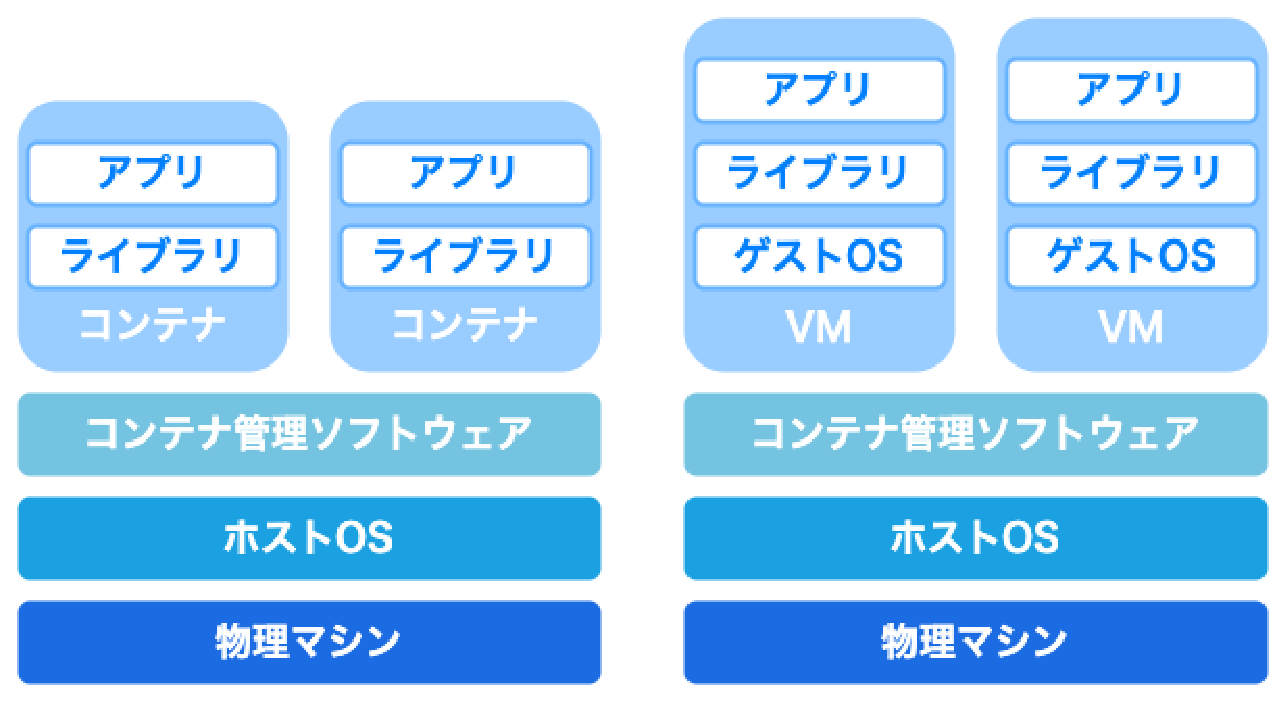
\includegraphics[width=\linewidth]{./fig/chap3/docker.eps}
    \hspace*{\fill}
    \caption{ハイパーバイザ型仮想化とコンテナを用いたOS仮想化}
    \label{docker}
\end{figure}

さらに,Dockerを利用することで様々な利点も生まれる.

まず,仮想化環境をコード化して管理する事で,どのような環境の上にでも同一の環境を作成する事ができるという点である.
Dockerでは仮想化環境の構築情報をコード化されたファイルとして管理する.
このファイルを保存し配布する事で特定の環境を再現し,複数のマシン上で全く同一の環境を作り出すことが可能となる.
この機能は,ソフトウェアの開発やテストなどで異なるマシンに同一の環境を作成し,その上でアプリケーションを動作させる必要のある場合などによく利用されている.

また,環境の作成や廃棄が簡単であることも利点の1つである.
複数のサーバを連携させて全体で1台のサーバであるかのように動作させるクラスタシステムを構築する場合も,Dockerイメージがあればそれを元に複数の環境(コンテナ)を起動できる.
この機能を活用することにより開発環境,動作環境をはじめから作る必要がなくなり,クラスタシステムを構築することも容易になる.
さらに,Kubernetes \cite{k8s}などが有するコンテナオーケストレーションシステムを用いてクラスタ環境を管理することもできる.

\section{MDのコンテナ化}
前節で紹介したような仮想化技術を用いることで,異なるマシンでもアプリケーションを同一の環境で動作させる事ができる.
この仮想化技術を用いて,2章で先行研究として紹介したSBCを用いたマルチディスプレイシステムを仮想化することを考える.

先行研究では,SBCマルチディスプレイシステムにおいてディスプレイノードとしてRaspberry Piを使用している.
2022年2月現在においてはSBCの開発が盛んに行われており,市場には数百種類ものSBCが存在している \cite{hackerbords}.
それらのSBCの間ではアーキテクチャ,OS,ディスプレイの描画方法,対応言語などに違いが存在する.
そのため,これらのSBCを用いてマルチディスプレイを構築する場合には構築の手順や動作に異なる点が生じることが予想される.
異なるSBCを用いた際に発生するこれらの差異を吸収するためには,様々なSBCに対応することができるマルチディスプレイ構築用ミドルウェアの開発が必要である.
そこで,前節で紹介したコンテナ仮想化技術であるDockerの利用を検討する.

\begin{figure}[H]
    \hspace*{\fill}
    \includegraphics[width=\linewidth]{./fig/chap3/md_docker.eps}
    \hspace*{\fill}
    \caption{Dockerを用いた環境構築}
    \label{docker_usage}
\end{figure}

Dockerを用いた環境構築の概要図を図\ref{docker_usage}に示す.
ユーザは,まずヘッドノードもしくはディスプレイノードとして利用するマシンに対してDockerのインストールを行う.
次に, Dockerに用意されているコマンドを用いてGitHub \cite{github}上のリポジトリからソースコードを取得し,その中に含まれているDockerfileを用いてホストマシン内にコンテナ環境を作成する.
ここでDockerfileとはコンテナ環境の構成情報 (OS,パッケージ,ネットワーク設定情報など) を保存したファイルであり,これを用いてコンテナ環境を構築することによりファイルによってあらかじめ設定されていた環境を簡単に構築することができる.
最後にホストマシン上に構成したコンテナ環境内でプログラムのビルドを行う事で,そのマシンをヘッドノードもしくはディスプレイノードとして使用することが可能になる.

\section{コンテナを通したディスプレイの制御}
本節では,コンテナ技術を用いて構築したMDにおけるフレーム表示時に生じる問題とその対処について説明する.
マシンに接続されたディスプレイに画像フレームを表示する際には,一般にフレームバッファとよばれる領域が使用される.
フレームバッファはマシンの/devディレクトリに存在するデバイスファイルである.
このファイルの中にディスプレイに表示するデータを格納することで,OSがディスプレイに画像を描画するという仕組みになっている.
フレームバッファを用いたディスプレイへの画像表示の概要を図\ref{framebuffer}に示す.

\begin{figure}[H]
    \hspace*{\fill}
    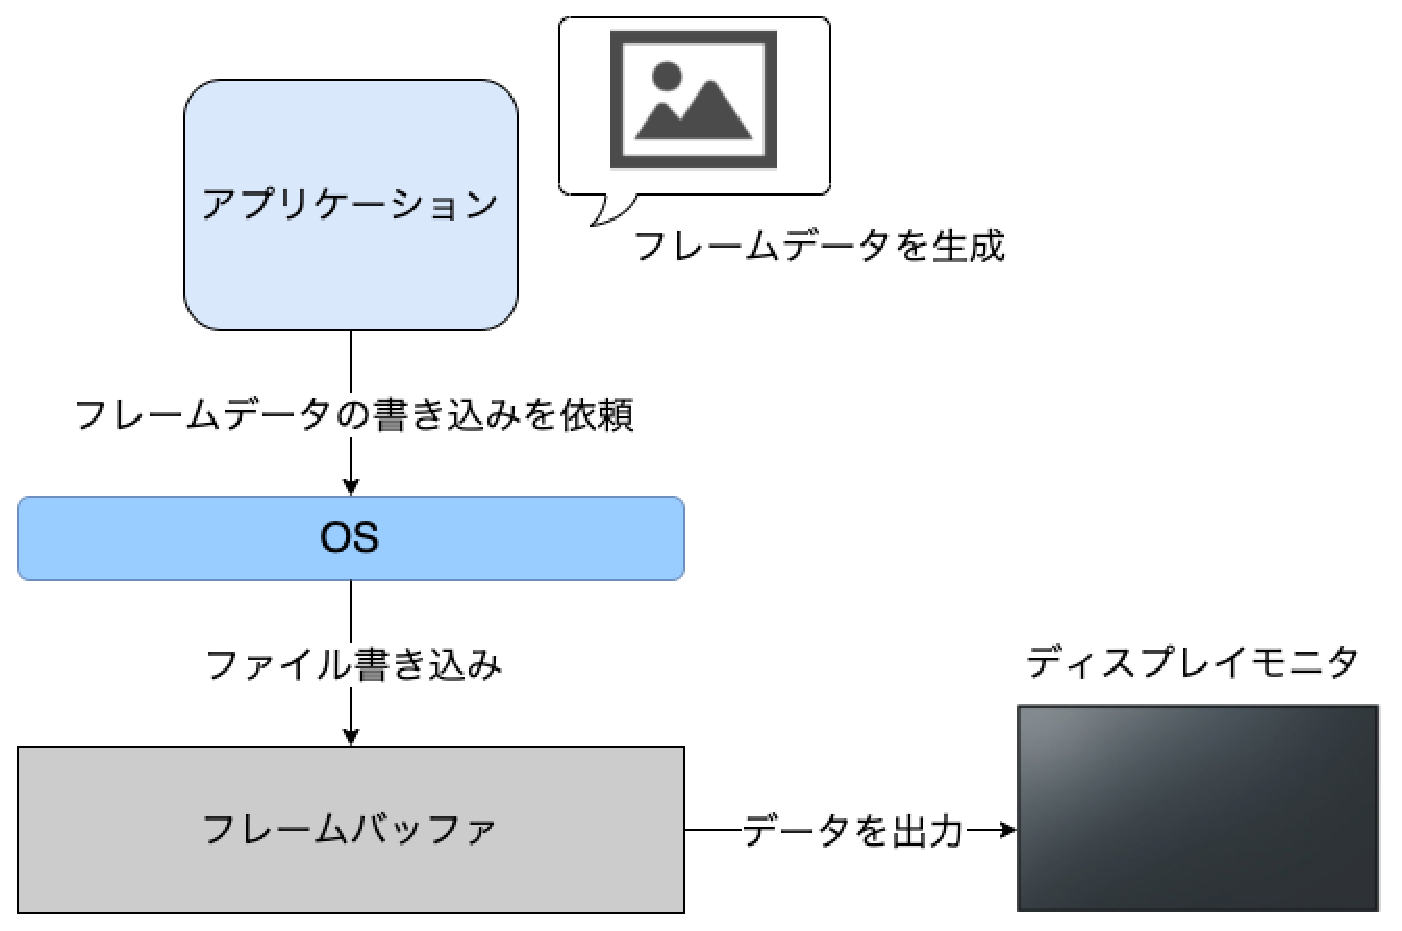
\includegraphics[width=\linewidth]{./fig/chap3/framebuffer.eps}
    \hspace*{\fill}
    \caption{フレームバッファを用いたディスプレイ表示}
    \label{framebuffer}
\end{figure}

Dockerを用いて構築したコンテナ環境の内部からは,ホストマシンのリソースへのアクセスが制限される場合がある.
例えば,デフォルトの状態ではDockerコンテナはDockerコンテナの内部でDockerデーモンの起動を行うことができない.
これは、デフォルトではコンテナからホストマシンのデバイスへのアクセスが許されていないことが原因である.
同様に,フレームバッファもDockerコンテナの内部から見ればホストマシン内のデバイスファイルであるため,ファイルが操作できずに画像フレームデータをディスプレイへの表示することができなくなっている.
この状態を,コンテナはunprivilegedな状態であるという.

対して,privilegedなコンテナはホストマシンの全てのリソースにアクセスする事ができる.
コンテナをpriviledgeな状態で起動するためには,起動時のコマンドで--privilegedコマンドを指定する必要がある.

\section{ヘッドノードでのフレーム処理の改良}
ここまでに紹介した技術を用いることで,SBCマルチディスプレイシステムをコンテナ基盤上で動作させることができるようになる.
続いて本節以降では,本研究の提案の中心部分となるヘッドノードでのフレーム処理の改良について述べる.

2章でも説明した通り,先行研究で提案されたマルチディスプレイには高解像度な動画や高フレームレートな動画をMD上に表示しようとするとヘッドノードでの処理がボトルネックとなり,動画表示に遅延が発生するという問題点がある.
高解像度な動画はフレームの分割や圧縮にかかる時間が大きくなるためヘッドノード内での処理時間が増加し,フレームの表示処理への影響も大きくなる.
また,高フレームレートな動画の場合にはフレーム処理時間の影響により元々のフレームレートを維持したまま動画を表示することが困難になる.
さらに,大規模なMDを構築した際のパフォーマンス低下も問題点としてあげられる.
先行研究のMDではヘッドノード内でフレーム圧縮を行うスレッドが1つであるため,MDを構成するディスプレイ数が増加するのに伴ってスレッドでの処理負荷が増加する.
その結果,MDの大規模化に伴ってフレーム処理にかかる時間も増加し,動画再生時のフレームレートが低下する.

この問題に対して,提案手法ではヘッドノードでのフレーム処理を並列化したプロセスとして実装し,ヘッドノード内でのフレーム処理時間の短縮を目指す.

\subsection*{フレーム処理のコンテナ並列化}
提案手法の実装にはOS仮想化技術を用いたコンテナ技術を使用し,プロセスレベルでの処理並列化を図る.
また,処理の並列化に伴うプロセス間での画像フレームの受け渡しについては,高速なプロセス間通信が可能な共有メモリを使用することでオーバーヘッドの低減を目指す.

先行研究では,ヘッドノード内の圧縮スレッド内でフレーム切り出し,フレーム分割,フレーム圧縮の3種類の処理が行われている.
フレーム切り出しとフレーム分割はディスプレイ数に関わらず1フレームに対して1回の処理のみが行われる.
しかし一方で,フレームの圧縮はマルチディスプレイを構成するディスプレイ数に応じて処理回数が変化する.
そのため,構成ディスプレイを増加させた場合にはこの部分がシステムのボトルネックとなる.
このボトルネックを解消するために,圧縮処理をヘッドノード内で並列化して行い,全体でのフレーム処理時間の短縮を試みる.

\begin{figure}[H]
    \hspace*{\fill}
    \includegraphics[width=\linewidth]{./fig/chap3/process_parallelization.eps}
    \hspace*{\fill}
    \caption{フレーム処理の並列化}
    \label{process_para}
\end{figure}

図\ref{process_para}に,提案手法におけるヘッドノード内のコンテナ構成を示す.
提案手法ではヘッドノード内で行われる処理それぞれを単一のコンテナに分割し,画像フレームの切り出し・分割を行う分割コンテナ,フレームの圧縮処理を行う圧縮コンテナ,そしてディスプレイノードとの同期用通信を行う同期制御コンテナの3種類のコンテナとして実装する.
圧縮コンテナは構成ディスプレイと同じ数だけ用意し,ヘッドノード内で並列化してフレームの圧縮処理を行う.

\subsection*{コンテナ間でのフレーム受け渡し処理}

処理の並列化を目的としてフレームの分割を行うコンテナと圧縮を行うコンテナを分けたことにより,ヘッドノード内のコンテナ間で画像フレームの受け渡しを行う必要が生じる.
この処理によるオーバヘッドを抑えるために,高速なプロセス通信が可能な共有メモリ (System V IPC) \cite{kerrisk2010linux,linux_kernel}を使用する.

以下,共有メモリ (System V IPC) について簡単に説明する.
IPCとはプロセス間通信 (InterProcess Communication) の略であり,ユーザモードプロセスから

\begin{itemize}
    \item セマフォを利用した他のプロセスとの同期
    \item 他のプロセスとの間でのメッセージ送受信
    \item 他のプロセスとのメモリ領域の共有
\end{itemize}

などの操作を行う事ができる.

System V IPCは,現在ではLinuxを含むほとんどのUNIXシステムで使用できるようになっている.
IPCのデータ構造は,プロセスがIPC資源 (セマフォ,メッセージキュー,共有メモリリージョン) を要求した際に動的に作成される.
IPC資源を要求したプロセスが獲得した資源を明示的に解放しない限りIPC資源はメモリ上に残り続け,他のどのプロセスからでも使用できる状態になる.
各資源は,ファイルシステムツリーにおけるファイルのパス名に相当する32ビットのIPCキーによって識別される.
また,各IPC資源は32ビットのIPC識別子を持つ.
IPC資源はカーネルによって決定されるが,IPCキーは自由に決める事が可能である.
複数のプロセスがIPC資源を利用する際には,IPC識別子が利用される.
本研究の実装ではSystem V IPCを利用して共有メモリ領域を獲得し,異なるプロセス間でのデータ共有を高速に行うことを目的とする.

続いて,IPC資源の利用方法について説明する.
System V IPCを用いて共有メモリ領域を獲得するためには,shmget()関数を使用する.
shmget()関数は引数として渡されたIPCに対応するIPC識別子を取得し,そのIPC識別子を利用することでプロセスが共有メモリ領域にアクセスすることができるようになる.
別々のプロセスから同一のIPC資源を共有するための方法は2通り存在する.
1つはプロセス間であらかじめ固定のIPCキーを決定しておく方法である.
この方法は単純であるため,多くのプロセスが関連する複雑なアプリケーションで利用してもうまく動作する.
しかし,全く関係ないプロセスが偶然同じIPCキーを使用してしまう可能性がある.
もう1つは,一方のプロセスでIPCキーにIPC\_PRIVATEを指定する方法である.
この方法では新規のIPC資源が割り当てられ, そのIPC識別子によってアプリケーション内の他のプロセスとの通信を行うため,他のプロセスから誤ってIPC資源を利用されてしまうことを防げる.

以上の方式を検討した結果,本研究では複数のコンテナ間でのデータの受け渡し処理に使用することを想定しており,IPC資源が複数のプロセスから参照されることになるため,実装が容易になる前者の手法を採用した.

\subsection*{IPC共有メモリ}

IPC共有メモリでは,共有するデータ構造をIPC共有メモリリージョンに配置することにより,複数のプロセスから共有データ構造にアクセスする事ができる.
以下,IPC共有メモリの使用方法について述べる.
プロセス1とプロセス2の2つの異なるプロセスの間で共有メモリ領域を作成するメモリ領域を作成するとする.
まずプロセス1はプロセス2との間で一意となるIPCキーを作成する.
そして,このキーを用いてshmget()関数によりIPC識別子を取得する.
この時に,獲得する共有メモリ領域のサイズやパーミッションなどを決める事ができる.
続いて,IPC識別子を引数としてshmat()関数を実行することにより,共有メモリがプロセス1のメモリ領域にアタッチされ,プロセス1から共有メモリ領域へのアクセスが可能になる.

もう一方のプロセス2では,プロセス1が生成したIPCキーを取得する.
続いてプロセス1と同様に取得したIPCキーを引数としてshmget()関数を実行し,共有メモリのIPC識別子を取得する.
その後,IPC識別子を引数としてshmat()関数を実行して共有メモリをプロセス2のアドレス空間にアタッチすることでプロセス2からもプロセス1と同じ共有メモリ領域を使用することができるようになる.
以上に述べたような一連の手続きを行うことで,作成した共有メモリ領域を利用して異なるプロセスとの間でデータを共有することが可能になる (図\ref{shared_memory}).

\begin{figure}[H]
    \hspace*{\fill}
    \includegraphics[width=\linewidth]{./fig/chap3/ipc1.eps}
    \hspace*{\fill}
    
\end{figure}

\begin{figure}[H]
    \hspace*{\fill}
    \includegraphics[width=\linewidth]{./fig/chap3/ipc2.eps}
    \hspace*{\fill}
\end{figure}


\begin{figure}[H]
    \hspace*{\fill}
    \includegraphics[width=\linewidth]{./fig/chap3/ipc3.eps}
    \hspace*{\fill}
\end{figure}

\begin{figure}[H]
    \hspace*{\fill}
    \includegraphics[width=\linewidth]{./fig/chap3/ipc4.eps}
    \hspace*{\fill}
    \caption{共有メモリ使用の流れ}
    \label{shared_memory}
\end{figure}

\subsection*{フレーム受け渡し機能の実装}

続いて,フレーム受け渡し機能の具体的な実装について説明する.
共有メモリは,ヘッドノード内で動作する分割コンテナと圧縮コンテナとの間で画像フレームデータを共有するために利用する.
分割コンテナは,動画ファイルから画像フレームの切り出し処理を行う.
このとき,画像処理にはオープンソースのコンピュータビジョンライブラリであるOpenCVを使用する.
OpenCVにおいて画像フレームはMatという型で管理される.
Mat型は画像フレームに関するパラメータを持った構造体であり,画像フレームの縦横ピクセル数,画像フレームの色深度,画像フレームのデータへのポインタなどをメンバとして保持している.
Mat構造体の内容を図\ref{mat}に示す.

\begin{figure}[H]
    \hspace*{\fill}
    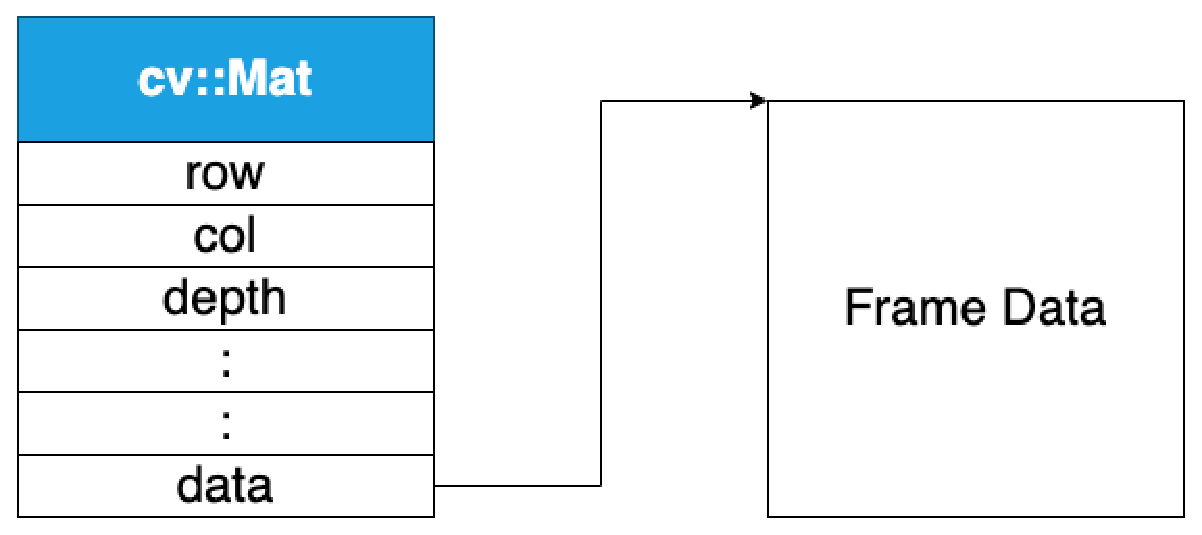
\includegraphics[width=\linewidth]{./fig/chap3/mat.eps}
    \hspace*{\fill}
    \caption{OpenCVにおけるMat構造体}
    \label{mat}
\end{figure}

プロセス間でのフレームデータ共有を行うためには,このMat型の構造体を共有メモリに格納し,プロセス間で共有できるようにすることが必要である.
しかし,Mat型の構造体を単純な操作で共有メモリに格納するだけではフレームデータそのものの受け渡しは実現できない.
これはMat構造体はフレームデータの実態ではなくデータ格納場所を指すポインタのみを保持しており,フレーム切り出しの際に画像フレームの画素データ本体が格納されるのはそのプロセスに固有のメモリ空間であるためである.
そこで本実装では,分割コンテナと圧縮コンテナとの間に作成した共有メモリ領域をchar型の配列として定義し,Mat構造体のもつフレームデータ格納場所へのポインタの値を利用してmemcpy()関数によるコピーを行っている.
memcpy()関数は引数を3つ持ち,引数1を先頭としたメモリ領域に,引数2を先頭としたメモリから引数3byte分のデータをコピーする.
memcpy()関数によるメモリのコピーは非常に高速に動作するため,共有メモリ領域への書き込みで生じるオーバーヘッドは小さくなる.

実際の処理では,まず分割コンテナがフレームの切り出しと分割を行った後,圧縮コンテナとの間に作成された共有メモリにフレームデータを格納する.
圧縮コンテナは共有メモリに格納されたフレームを取得し,圧縮処理を行う.

共有メモリはヘッドノードの中に1つのみを作成し,その中でそれぞれの圧縮コンテナに対してメモリ領域を分割して割り当てるという手法を採用する.
また,共有メモリにはフレーム切り出しの際に使われるOpenCVのMat形式を文字型の配列に変換してからフレームデータを格納する(図\ref{shared_memory2}).

\begin{figure}[H]
    \hspace*{\fill}
    \includegraphics[width=\linewidth]{./fig/chap3/shared_memory2.eps}
    \hspace*{\fill}
    \caption{共有メモリの使用例2}
    \label{shared_memory2}
\end{figure}

\subsection*{フレーム受け渡し処理の詳細}

続いて,共有メモリ領域を用いたフレームデータの受け渡しについて詳細な動作を説明する.
フレームデータ受け渡しに用いる共有メモリ領域は,はじめに分割ノードによってホストマシン内に1つだけ作成される.
その1つの共有メモリ領域に対して分割メモリはフレームデータの格納を行う.
接続ディスプレイと同数だけ用意された全ての圧縮コンテナは1つの共有メモリに対してデータの取り出しを行う.
また,作成したメモリの共有を行うには共有メモリを作成した際に使用されたIPCキーを分割ノードと圧縮ノードとの間で共有する事が必要になる.
このIPCキーの共有にはホストマシンのメモリ領域を利用している.
まず,分割ノードにより共有メモリの作成に使用されたIPCはあらかじめ設定されたパスに存在する物理マシン内のテキストファイルに文字列として保存される.
その後起動された圧縮コンテナが物理マシン内の該当パスに存在するフォルダを認識し,その中に記述されているIPCキーを引数としてコンテナ内でプログラムを実行する.
この仕組みによって分割コンテナと圧縮コンテナとの間でIPCキーを共有することができ,同一のメモリ領域にアクセスする事が可能になる.

\begin{figure}[H]
    \hspace*{\fill}
    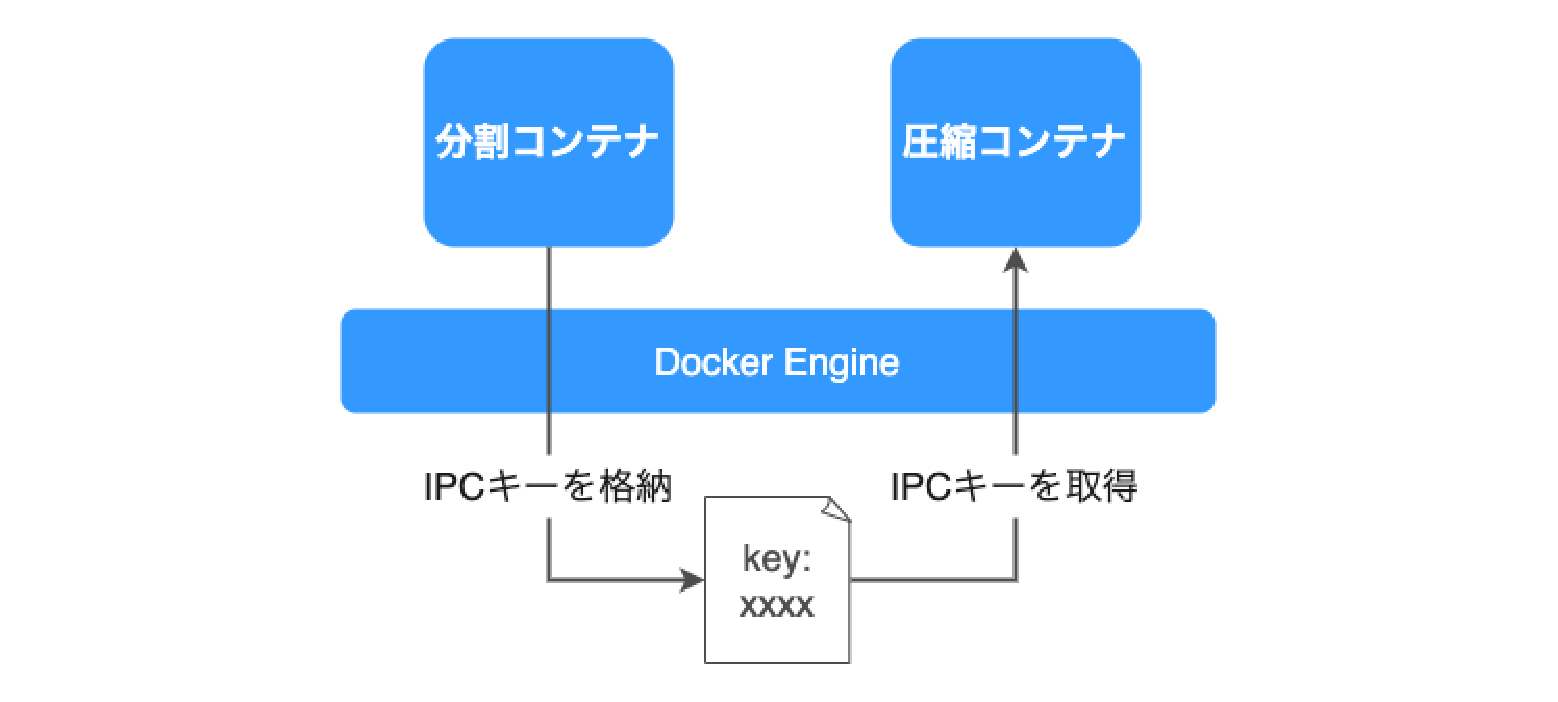
\includegraphics[width=\linewidth]{./fig/chap3/ipckeyshare.eps}
    \hspace*{\fill}
    \caption{共有メモリの使用例2}
\end{figure}

共有メモリ領域では,フレームの格納および取り出しを高速で行うために,分割コンテナによって格納された分割済みの画像フレームデータをバッファリングする仕組みを用意する.
共有メモリに格納される画像フレームデータは,ディスプレイノードが接続しているディスプレイと同じ解像度となる.
本研究では,動画の表示に使用されるディスプレイモニタの解像度としてFull HD (1920 x 1080ピクセル) のものを想定する.
また,色深度は赤,緑,青の3深度とする.
この想定下では,共有メモリに格納される分割後の画像フレームは1920 x 1080ピクセル,色深度3, ビット深度 (1ピクセル,1色のデータを保持するのに必要なビット数)8となり,そのデータ量はおよそ5.9MBとなる.
よって,各圧縮コンテナに対して8枚の分割済みフレームをバッファリングするとすると,必要な共有メモリの領域は(圧縮コンテナ数) x 5.9 x 8 (MB) で算出することができる.
例えば,4面構成のマルチディスプレイを構築する場合には約189MB, 9面構成のマルチディスプレイを構築する場合には約425MBの共有メモリ領域が必要となる.
このメモリ領域を,分割コンテナは起動と同時に獲得する処理を行う.

分割コンテナは,新たなフレームの切り出しを行いそれに対する分割処理を完了すると,共有メモリ領域に用意されたバッファに順次フレームを格納していく.
バッファにはそれぞれの圧縮コンテナに対して領域を定めておき,圧縮コンテナはその領域から順番にフレームの取り出しを行い後続の処理を開始する.
共有メモリ領域に作成されたバッファを用いてコンテナ間で画像フレームの受け渡しを行う様子を,図\ref{buffer}に示す.

\begin{figure}[H]
    \hspace*{\fill}
    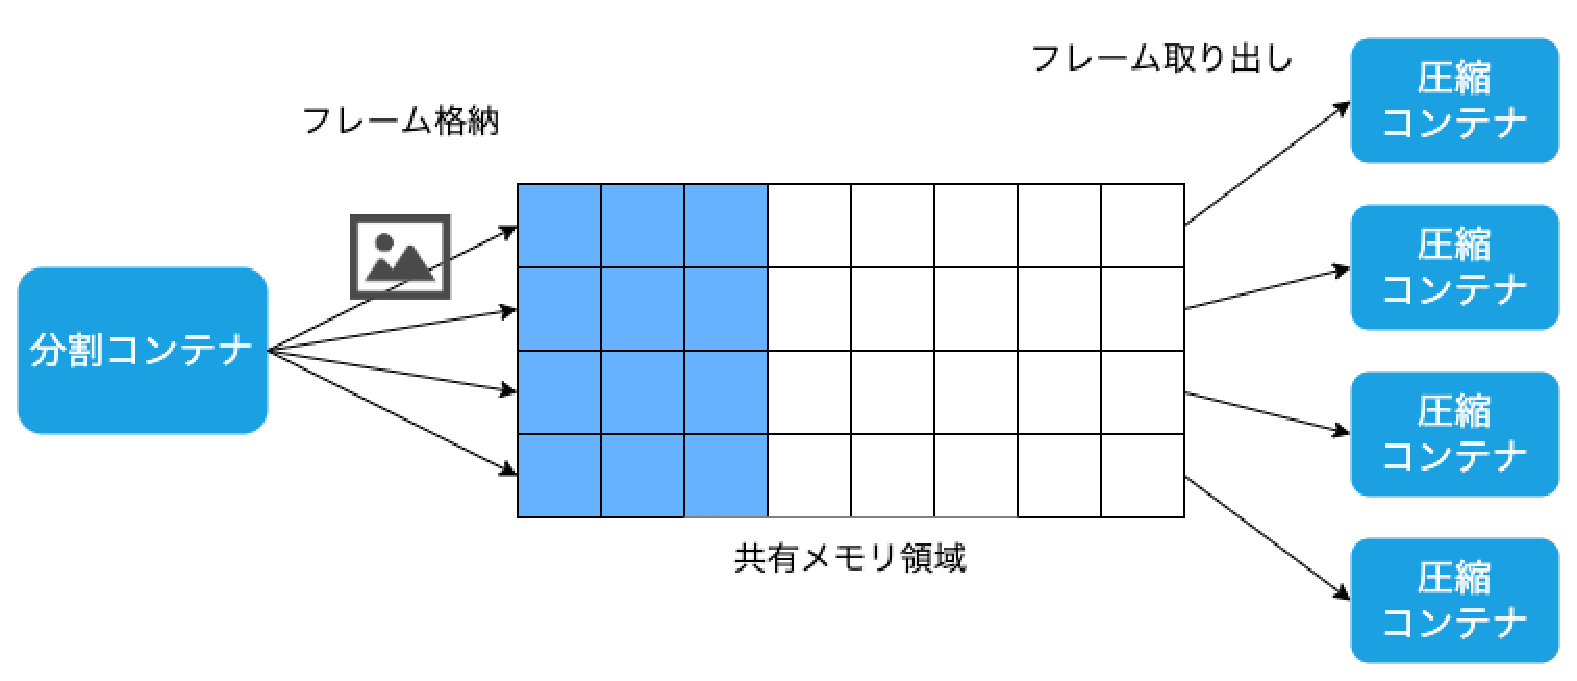
\includegraphics[width=\linewidth]{./fig/chap3/buffering.eps}
    \hspace*{\fill}
    \caption{共有メモリ内におけるフレームのバッファリング}
    \label{buffer}
\end{figure}

\subsection*{各コンテナでの処理}
ここでは,各コンテナ内での処理について順に述べる,
図\ref{divide_container}および図\ref{compress_container}に提案手法における分割コンテナと圧縮コンテナの処理フローチャートを示す.

\begin{figure}[H]
    \hspace*{\fill}
    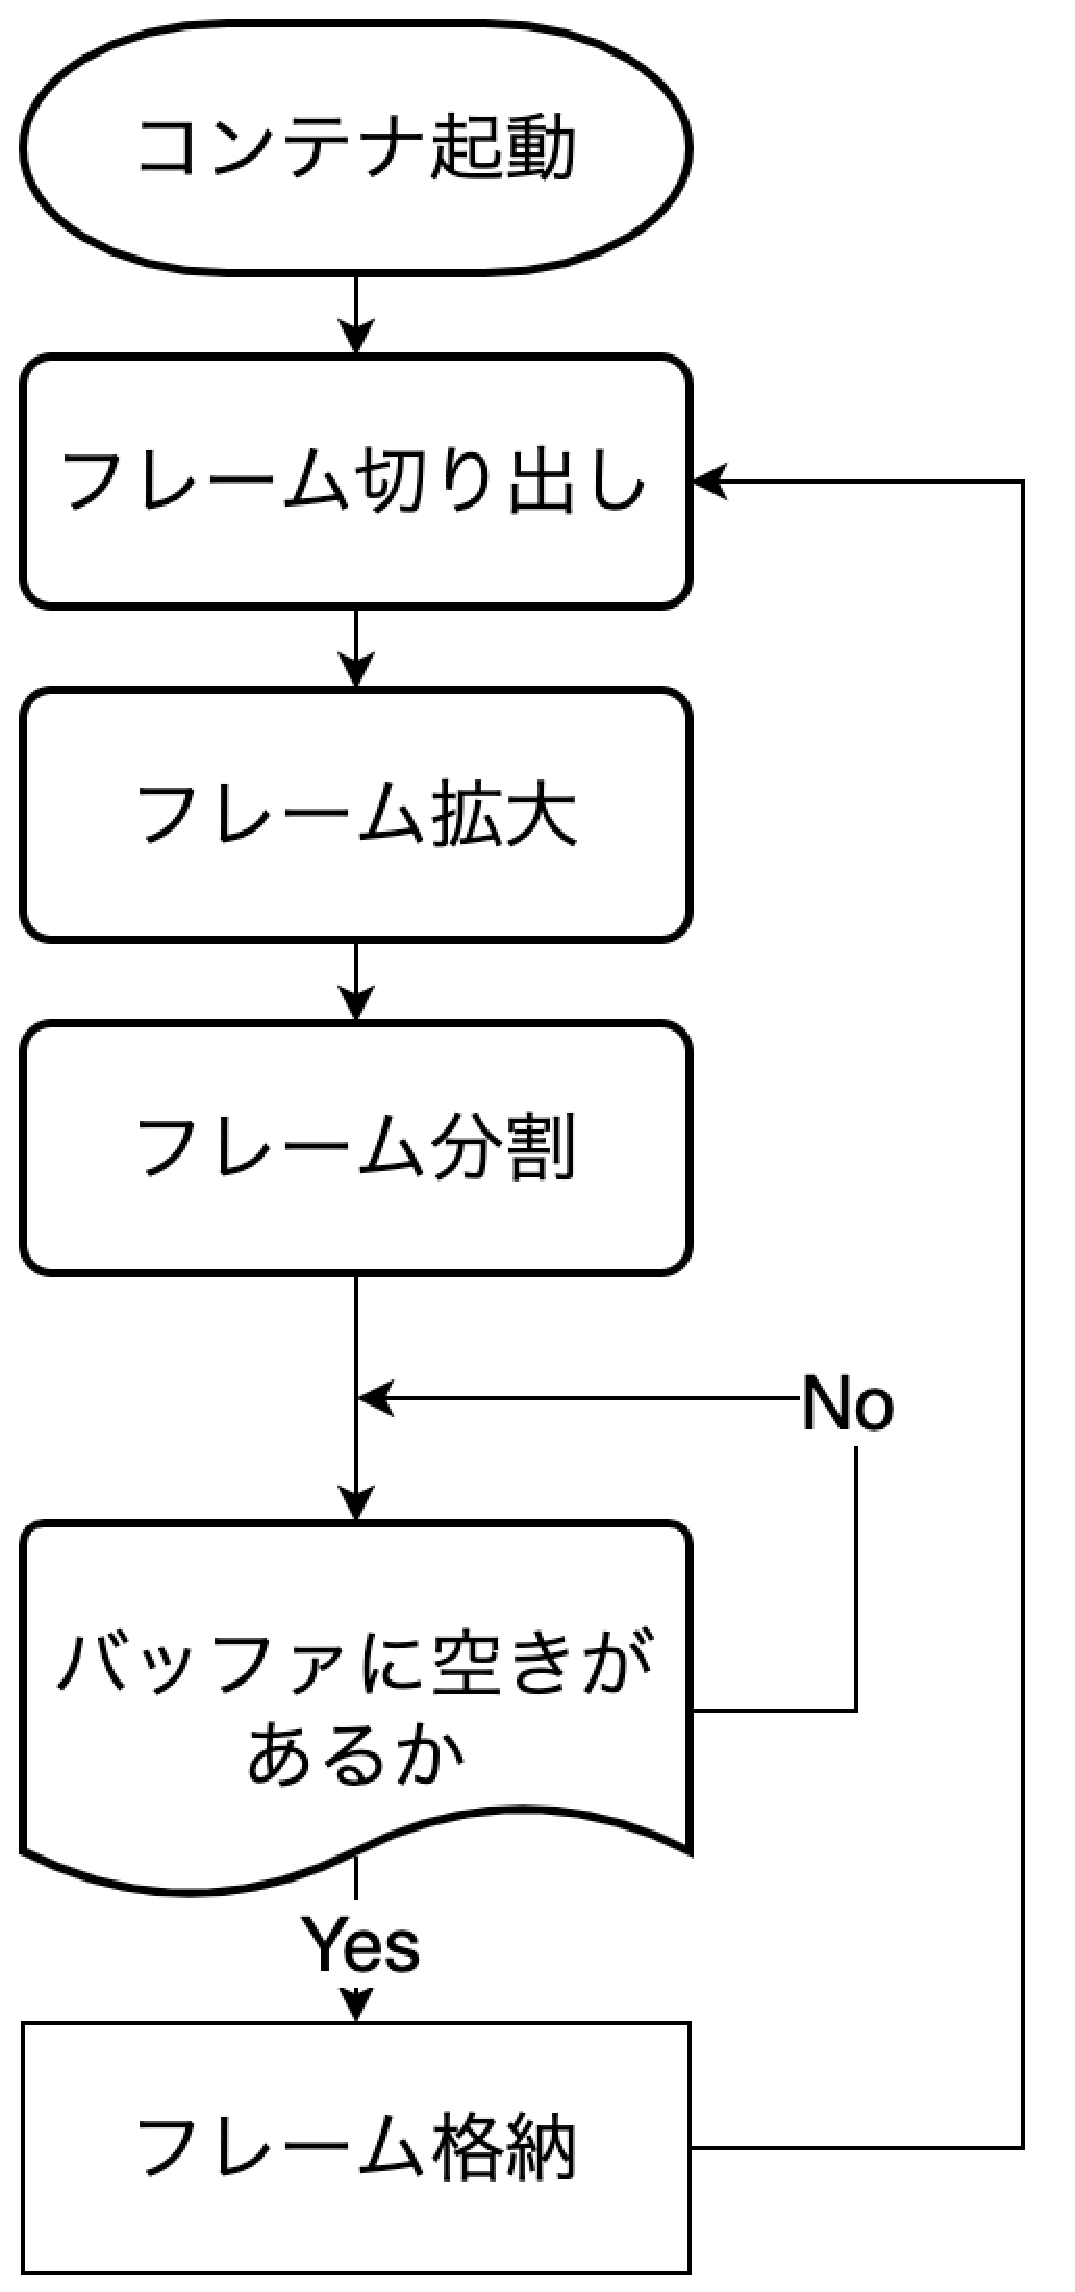
\includegraphics[width=60mm]{./fig/chap3/bunkatu_flow.eps}
    \hspace*{\fill}
    \caption{分割コンテナの動作フロー}
    \label{divide_container}
\end{figure}

分割コンテナは,コンテナが起動されるとすぐに動画ファイルからのフレーム切り出し処理を開始する.
その後,切り出したフレームに対して,構築したマルチディスプレイの解像度に応じたサイズにフレームの拡大処理を行う.
次に,ディスプレイの数に応じた分割処理を行い,共有メモリに作成されたバッファに順に格納していく.
このとき,共有メモリ内のバッファにはあらかじめ用意したバッファの数以上のフレームを格納する事ができない.
そのため,フレームの格納処理を行う前にバッファに格納されているフレーム数を取得し,バッファ上にあるフレーム数が上限に達していれば格納処理を行わずに待機状態になる.
その後,圧縮フレームがバッファから画像フレームを取り出すことによってバッファに空きができたことを認識すると待機状態を終了し,現在処理中のフレームデータを格納して次のフレームの処理へと移る.

\begin{figure}[H]
    \hspace*{\fill}
    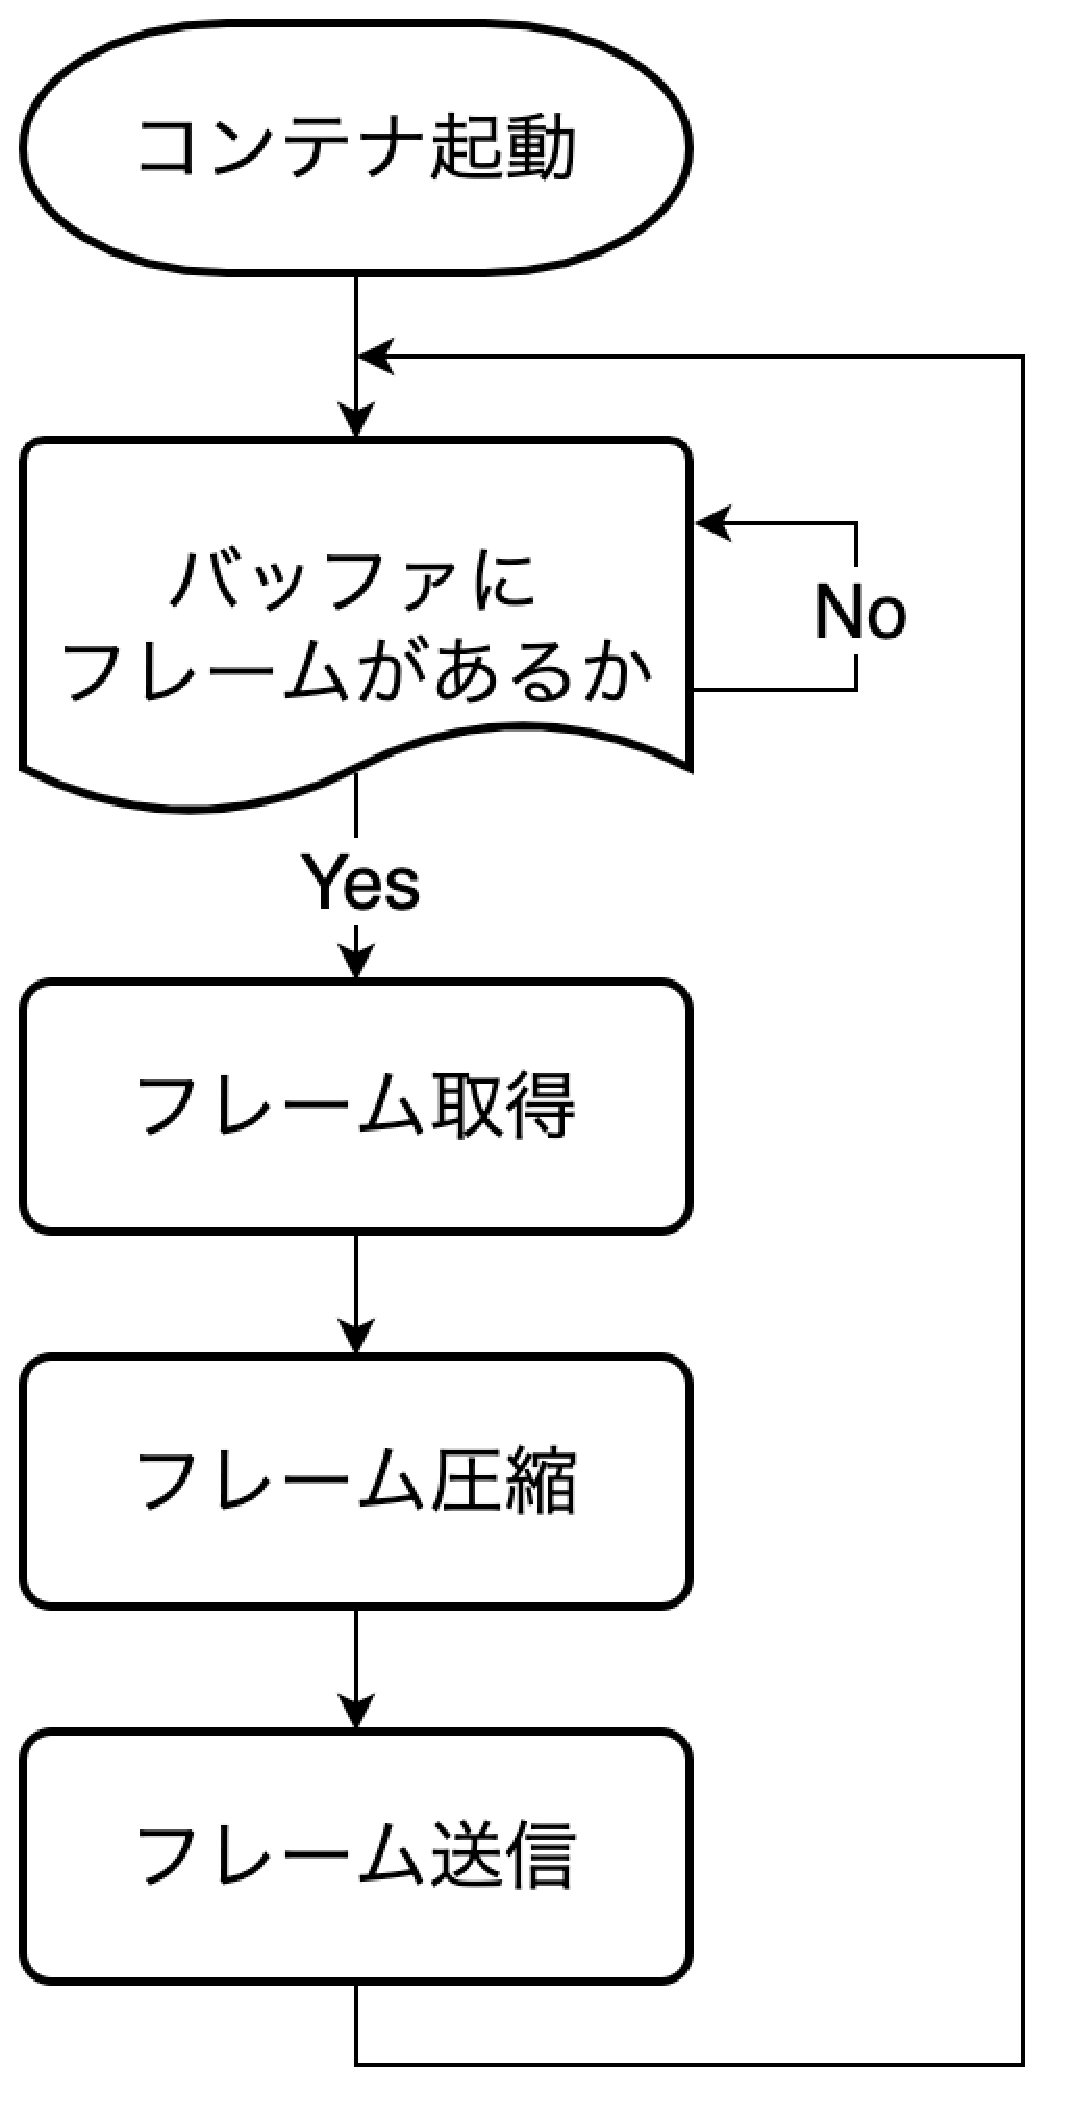
\includegraphics[width=60mm]{./fig/chap3/assyuku_flow.eps}
    \hspace*{\fill}
    \caption{圧縮コンテナの動作フロー}
    \label{compress_container}
\end{figure}

圧縮コンテナは起動と同時に分割コンテナとの共有メモリを取得し,バッファにフレームが格納されているかどうかの監視を開始する.
分割コンテナによってバッファに分割済みの画像フレームが格納されたことを確認すると監視を終了し,フレーム処理を開始する.
圧縮コンテナで行われるフレーム処理は,フレームの圧縮と送信である.
バッファから画像フレームを取り出して圧縮処理を行うと,OpenCVのMat形式から文字列オブジェクト (C++のstring型) への変換が行われる.
この文字列オブジェクトを接続したディスプレイノードへと送信するまでが各フレームに対する一連の処理となる.

\subsection*{提案手法を用いたマルチディスプレイシステムの構築}
最後に,提案手法を用いて構築したマルチディスプレイの全体像について述べる.
図\ref{system_flow_teian}に提案手法を用いて構築したMDの動作フローを示す.
ヘッドノードでは分割コンテナ,圧縮コンテナ,同期制御コンテナの3種類のコンテナが動作している.
処理の流れとしては,まず分割コンテナが動画ファイルから1フレームずつ切り出し,構成ディスプレイ数に応じて分割処理が行われた後,作成した共有メモリ領域に格納する.
圧縮コンテナは,共有メモリから分割済みの画像フレームを取得する.
圧縮コンテナはこのフレームに対してJPEG圧縮処理を行い,それぞれが接続しているディスプレイノードへの送信処理を行う.
圧縮コンテナからフレームを受け取ったディスプレイノードではフレーム展開処理を行い,展開後の画像フレームをホストマシンのフレームバッファに書き込むことでディスプレイへ画像を表示する.
この処理を各フレームに対して行うことで接続されたディスプレイ上への動画の再生が実現される.
また,ヘッドノードの内部では分割コンテナと複数の圧縮コンテナの他に同期制御コンテナも動作する.
同期制御コンテナの役割はディスプレイノードで動作している表示制御スレッドにフレームの表示命令を送信することである.
同期制御スレッドはディスプレイノードから各画像フレームが表示バッファに格納され,ディスプレイの表示準備が完了した旨の通知を受け取る.
この通知が全てのディスプレイノードから送信されたことを確認し,同期制御スレッドが各ディスプレイノードに対してフレームの表示命令を送信する.
さらに,同期制御スレッドは圧縮コンテナ内で行われているフレーム圧縮のパラメータを制御することでフレームレートを一定に保つ役割を持つ.


\begin{figure}[H]
    \hspace*{\fill}
    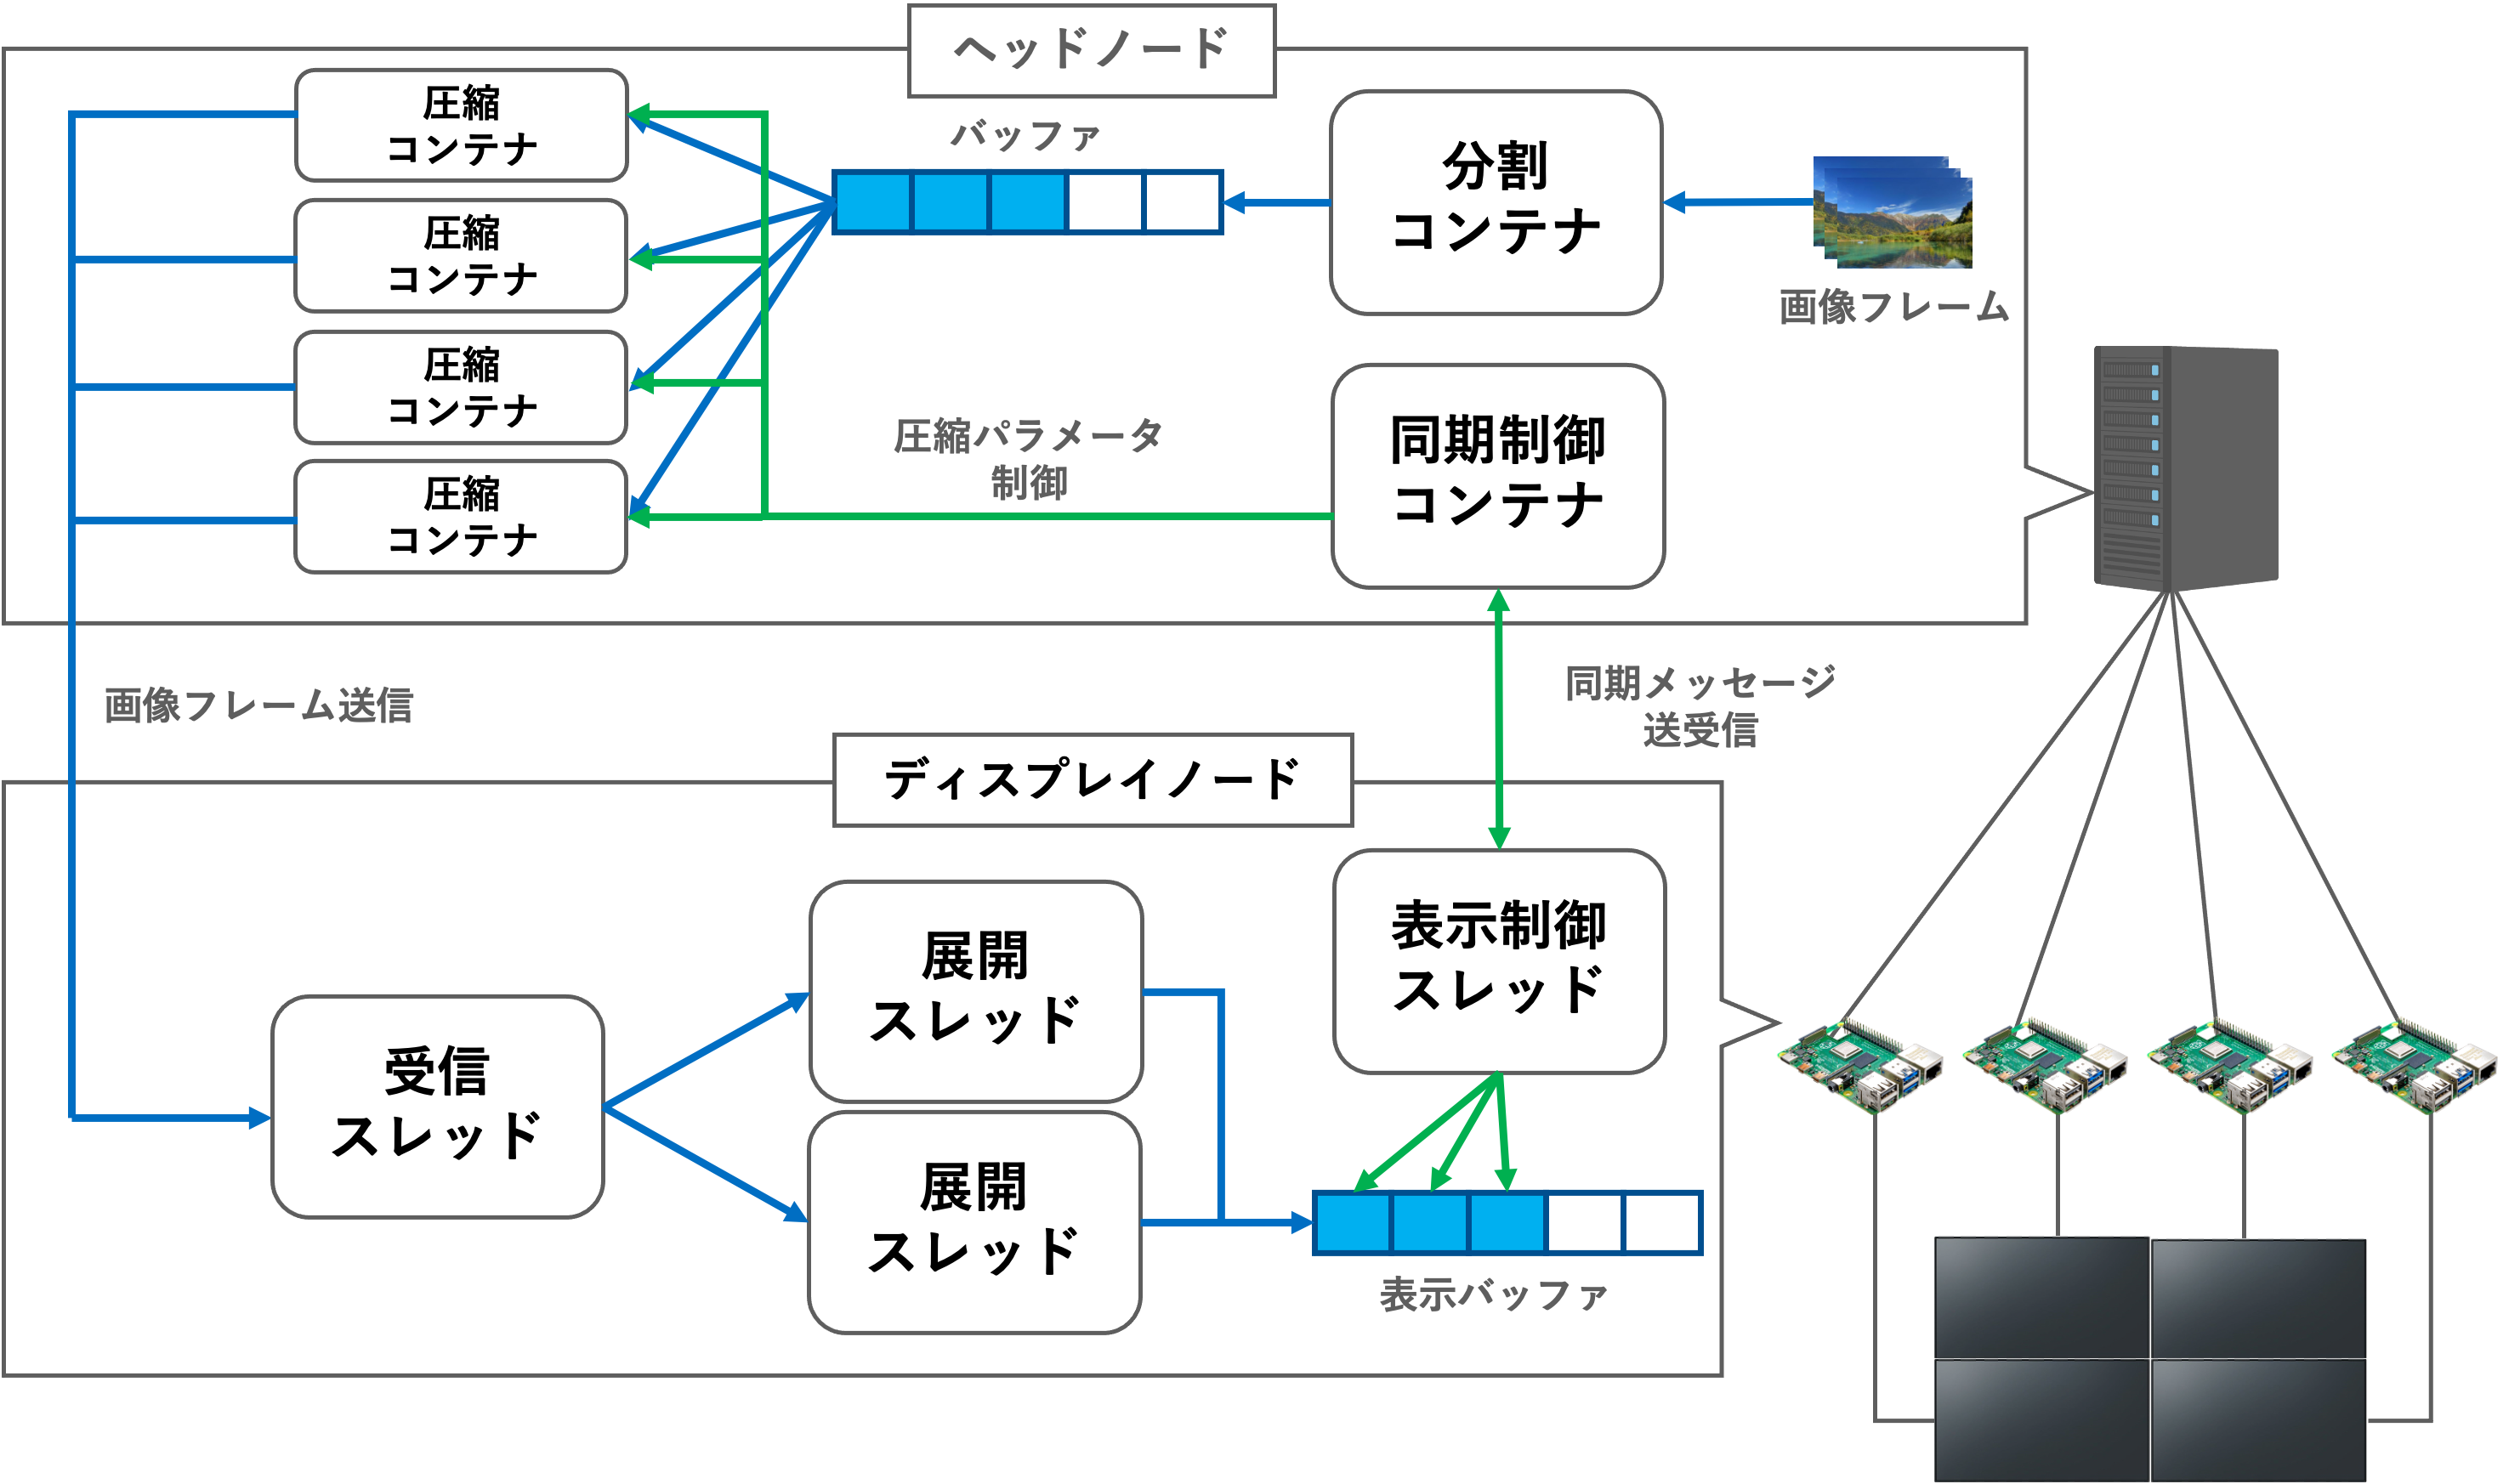
\includegraphics[width=\linewidth]{./fig/chap3/system_flow.eps}
    \hspace*{\fill}
    \caption{提案手法を用いたMDの動作フロー}
    \label{system_flow_teian}
\end{figure}


\chapter{評価}
行った評価の内容について簡単に説明する

\section{実験環境}
実験環境について書く
使用機器,使用ネットワーク帯域,使用動画ファイル,OS,モジュールなど

\begin{table}[H]
    \caption{ヘッドノード用デスクトップPCの仕様}
    \begin{center}
    \begin{tabular}{cc}
    \hline
    要素 & 仕様 \\\hline\hline
    CPU & i7-5960X (3.0 GHz×8) \\ \hline
    メモリ & 64.0 GB \\ \hline
    通信帯域 & 1 Gbps \\ \hline
    OS & CentOS 7.3 \\ \hline

    \end{tabular}
    \end{center}
\end{table}

評価に用いる映像としては,クリエイティブ・コモンズ・ライセンスのもとで利用できる3DアニメーションであるBig Buck Bunny \cite{bigbackbunny}を使用した.
表4.4に,Big Buck Bunnyのプロパティを示す.さらに,図4.3にBig Buck Bunny再生時のスクリーンショットを示す.

\begin{table}[htbp]
    \caption{Big Buck Bunnyのプロパティ}
    \begin{center}
    \begin{tabular}{cc}
    \hline
    項目 & 内容 \\\hline\hline
    動画形式 & MP4 \\ \hline
    コーデック & H.264 \cite{h264} \\ \hline
    長さ & 10分34秒 \\ \hline
    総フレーム数 & 19020枚 \\ \hline
    フレームレート & 30 fps \\ \hline
    解像度 & 4K (3840×2160) \\ \hline

    \end{tabular}
    \end{center}
\end{table}

\begin{figure}[H]
    \hspace*{\fill}
    \includegraphics[width=\linewidth]{./fig/bigbuckbunny.eps}
    \hspace*{\fill}
    \caption{Big Buck Bunnyのスクリーンショット}
   \end{figure}

ヘッドノードで行われる処理の実装には,OpenCV \cite{opencv}, libjpeg-turbo ~\cite{libjpeg}, Boost.Asio \cite{asio}という3種類のライブラリを利用した. 
OpenCVは画像処理ライブラリ,libjpeg-turboはJPEGの圧縮と展開を行うライブラリ,Boost.Asioはソケット通信を行うライブラリである.
また,ディスプレイノードの処理の実装にはlibjpeg-turbo, Boost.Asio, fbdevを利用した.
実装にはC++言語を使用し,GCCコンパイラ (GNU C Compiler) \cite{gcc}でコンパイルを行った.

\begin{figure}[H]
    \hspace*{\fill}
    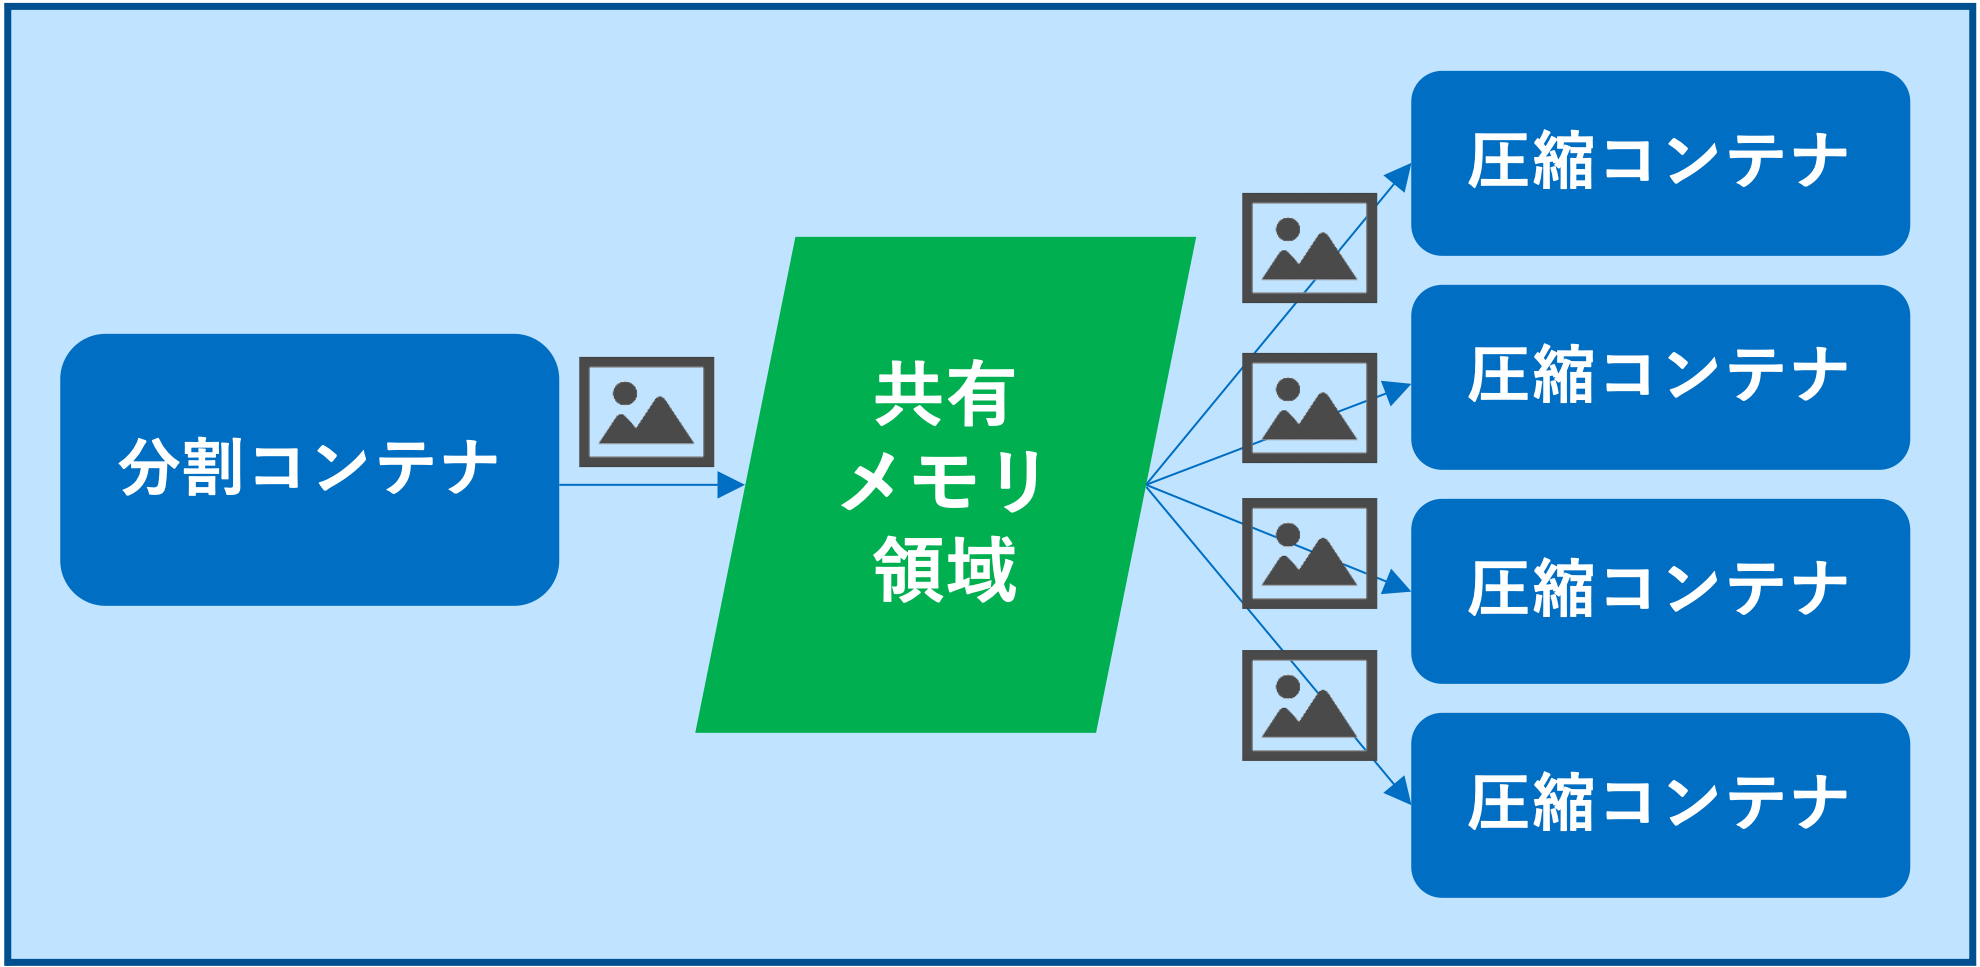
\includegraphics[width=\linewidth]{./fig/evaluation_environment.eps}
    \hspace*{\fill}
    \caption{実験環境のコンテナ構成}
   \end{figure}

\section{フレーム処理時間の評価}

\subsection{実験方法}
先行研究で提案された手法と提案手法において,4面構成のMDを想定した環境で4K解像度の画像を表示し,動画のフレーム開始から1000フレーム目の処理が終了するまでの1フレームあたりに要するフレーム処理時間を計測した.
図4.6に先行研究で提案されたシステムと提案手法でのフレーム処理時間を示す.

\subsection{実験結果}

既存手法ではヘッドノードでのフレーム処理時間の平均が52.35msであったのに対し,提案手法では21.72msとなっており,フレーム処理時間が既存手法と比較して40\%程度まで短縮された事が確認できた.

また,本提案で新たに生じた処理である共有メモリを用いたプロセス間での画像フレームデータ受け渡しに要する時間も平均で1ms未満となっており,オーバーヘッドは非常に小さくなっていることも確認できる.

以上の結果より,フレーム処理プロセスの並列化を行った提案手法によって,システムのボトルネックが解消された.

\begin{figure}[H]
    \hspace*{\fill}
    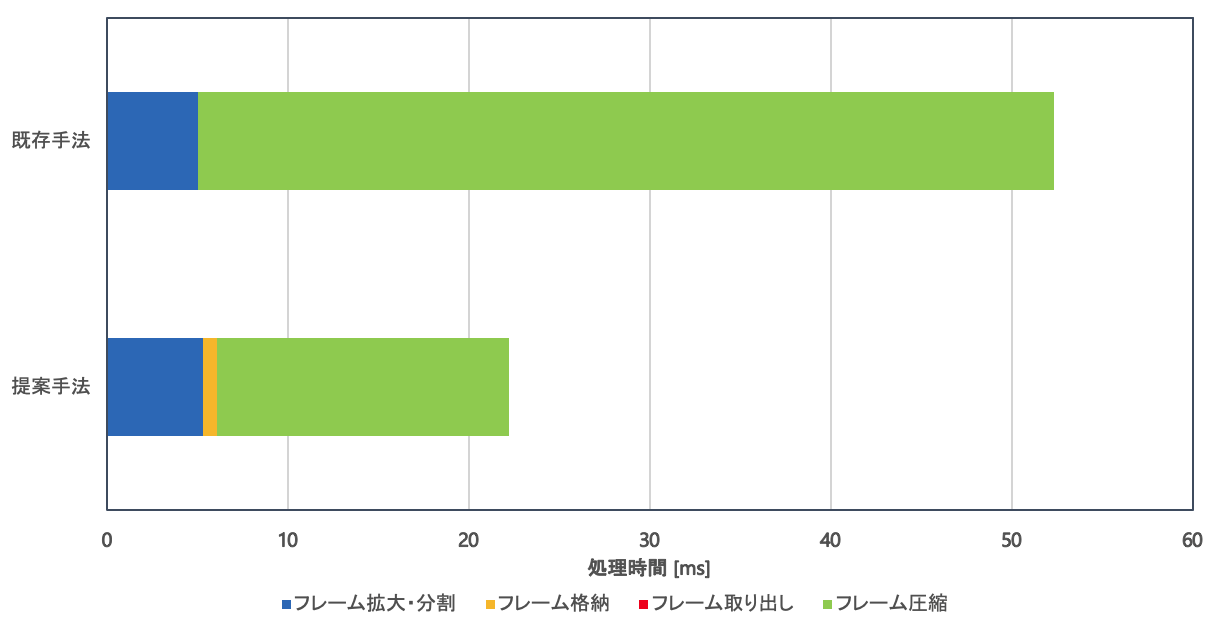
\includegraphics[width=\linewidth]{./fig/processing_time_evaluation_4k.eps}
    \hspace*{\fill}
    \caption{フレーム処理時間の比較}
   \end{figure}

\section{フレーム処理速度の評価}



\subsection{実験方法}

\subsection{実験結果}

\subsection{結果に対する考察}

\chapter{関連研究}

本章では,本研究と同様に,仮想化技術を用いてマルチディスプレイシステムを構築した関連研究をいくつか紹介し,その特徴について説明する.

大規模ディスプレイシステムにおいて動画再生時のフレームレート向上を試みた例としては,Bundulisらの研究 \cite{bundulis2018infiniviz}がある.Bundulisらは,以前にInfiniviz \cite{bundulis2016infiniviz}とよばれる大規模ディスプレイシステムを提案している.Infinivizは,仮想マシンベースの高解像度ディスプレイウォールシステムであり,既存の他の大規模ディスプレイしシステムと比較して,ネットワーク帯域幅の消費量と計算性能を向上させようとするものである.また,シームレスな方法で可視化タスクにアプローチし,大規模な高解像度ディスプレイウォール上で,一般的なデスクトップオペレーティングシステムのソフトウェアを変更することなく実行できるようにすることを目的としている.Bundulisらの研究では,Quake 3 Arena \cite{quake3arena}を解像度9600x5400, 24fpsで動作させた際のInfinivizの実際の性能を計測した.この研究では,仮想化を利用することで,ソフトウェアに依存しない仮想マシンベースの高解像度ディスプレイウォールシステムを構築している.

\begin{figure}[H]
    \hspace*{\fill}
    \includegraphics[width=90mm]{./fig/chap5/Infiniviz.eps}
    \hspace*{\fill}
    \caption{Infinivizのアーキテクチャ}
\end{figure}

\clearpage

Liuらは,DockerとGPUを利用して、画像、動画、WebGLアプリケーションなどを表示する大画面ビジュアライゼーションアプリケーションをデプロイする手法を提案している \cite{Liu_2019}.
この研究では,Dockerクラスタを構築して28個のコンテナを含むマイクロサービスを起動し,Unix/Linuxユーザにグラフィカルなインタフェースを提供するために広く使用されているX11Unixソケットをマッピングすることで大画面可視化システムをデプロイした.
同時に,アプリケーションをローカルホストで動作させた場合と比較し,性能を検証し,彼らの手法を大画面ビジュアライゼーションに適用した場合,許容できる性能劣化で良好な結果を得ることができると結論付けている.

\begin{figure}[H]
    \hspace*{\fill}
    \includegraphics[width=\linewidth]{./fig/chap5/docker_cluster.eps}
    \hspace*{\fill}
    \caption{Dockerクラスタを用いて構築したマルチディスプレイのトポロジ}
\end{figure}

\chapter{結論}

\section{本研究の総括}
本研究では,先行研究で提案された,ディスプレイノードにSBCを用いたマルチディスプレイに対して,ヘッドノード内でのフレーム処理時間を短縮しマルチディスプレイのスケーラビリティの向上を目指し,OS仮想化技術を用いたフレーム圧縮処理の並列化を提案した.


本研究の評価では,提案手法の効果を検証するために,

\section{将来課題}

\acknowledgement
本研究を行うにあたり,懇切なる御指導,御鞭撻を賜りました大阪大学サイバーメディアセンター応用情報システム研究部門 下條真司教授に心より感謝の意を表します.

本研究の全過程を通じ,研究の方向性検討や論文の執筆等,熱心な御指導,御鞭撻を賜りました大阪大学サイバーメディアセンター応用情報システム研究部門 木戸善之講師に心より感謝申し上げます.

本研究の進行から論文執筆まで多岐にわたり,手厚い御指導,御鞭撻を賜りました大阪大学サイバーメディアセンター応用情報システム研究部門 伊達進准教授,小島一秀講師に心より感謝の意を表します.

日頃より,丁寧かつ熱心な御指導を賜りました大阪大学情報推進本部 大平健司准教授に心より感謝の意を表します.

本研究において,厳しくも優しい御指導を賜りました大阪大学データビリティフロンティア機構サービス創出・支援部門 春本要教授に感謝の意を表します.

最後に,日々御支援と心からの激励をかけて頂いた下條研究室の皆様並びに事務補佐員 片岡小百合氏に心より感謝致します.


\bibliography{sample.bib}
\bibliographystyle{junsrt}

\end{document}

